\documentclass[12pt]{iopart}

\usepackage[T1]{fontenc}%
\usepackage{graphicx}%
\makeatletter
\@ifundefined{equation*}{}{%
  \expandafter\let\csname equation*\endcsname\@undefined
  \expandafter\let\csname endequation*\endcsname\@undefined}%
\makeatother
\usepackage{amsmath}%
\usepackage{amssymb}%
\usepackage{amsfonts}%
\usepackage{mathrsfs}%
\usepackage{bm}%
\usepackage{xcolor}%
\usepackage{textcomp}%
\usepackage{booktabs}%
\usepackage{array}%
\usepackage{newunicodechar}%
\providecommand{\tightlist}{\setlength{\itemsep}{0pt}\setlength{\parskip}{0pt}}
\providecommand{\texorpdfstring}[2]{#1}
\providecommand{\passthrough}[1]{#1}
\providecommand{\pandocbounded}[1]{#1}
\providecommand{\lt}{<}\providecommand{\gt}{>}
\newunicodechar{§}{\S}
\newunicodechar{→}{\ensuremath{\rightarrow}}
\newunicodechar{↔}{\ensuremath{\leftrightarrow}}
\newunicodechar{×}{\ensuremath{\times}}
\newunicodechar{·}{\ensuremath{\cdot}}
\newunicodechar{⊃}{\ensuremath{\supset}}
\newunicodechar{⊂}{\ensuremath{\subset}}
\newunicodechar{∘}{\ensuremath{\circ}}
\newunicodechar{°}{\ensuremath{^{\circ}}}
\newunicodechar{₀}{\textsubscript{0}}\newunicodechar{₁}{\textsubscript{1}}%
\newunicodechar{₂}{\textsubscript{2}}\newunicodechar{₃}{\textsubscript{3}}%
\newunicodechar{₄}{\textsubscript{4}}\newunicodechar{₅}{\textsubscript{5}}%
\newunicodechar{₆}{\textsubscript{6}}\newunicodechar{₇}{\textsubscript{7}}%
\newunicodechar{₈}{\textsubscript{8}}\newunicodechar{₉}{\textsubscript{9}}%
\newunicodechar{⁰}{\textsuperscript{0}}\newunicodechar{¹}{\textsuperscript{1}}%
\newunicodechar{²}{\textsuperscript{2}}\newunicodechar{³}{\textsuperscript{3}}%
\newunicodechar{⁴}{\textsuperscript{4}}\newunicodechar{⁵}{\textsuperscript{5}}%
\newunicodechar{⁶}{\textsuperscript{6}}\newunicodechar{⁷}{\textsuperscript{7}}%
\newunicodechar{⁸}{\textsuperscript{8}}\newunicodechar{⁹}{\textsuperscript{9}}%
\newunicodechar{⁻}{\textsuperscript{-}}\newunicodechar{≈}{\ensuremath{\approx}}%
\newunicodechar{≤}{\ensuremath{\le}}\newunicodechar{≥}{\ensuremath{\ge}}%
\newunicodechar{∼}{\ensuremath{\sim}}\newunicodechar{−}{\ensuremath{-}}%
\newunicodechar{–}{--}\newunicodechar{—}{---}%
\newunicodechar{∗}{\ensuremath{\ast}}\newunicodechar{∞}{\ensuremath{\infty}}%
\newunicodechar{∫}{\ensuremath{\int}}\newunicodechar{∝}{\ensuremath{\propto}}%
\newunicodechar{τ}{\ensuremath{\tau}}\newunicodechar{ν}{\ensuremath{\nu}}%
\newunicodechar{λ}{\ensuremath{\lambda}}\newunicodechar{σ}{\ensuremath{\sigma}}%
\newunicodechar{α}{\ensuremath{\alpha}}\newunicodechar{η}{\ensuremath{\eta}}%
\newunicodechar{β}{\ensuremath{\beta}}\newunicodechar{γ}{\ensuremath{\gamma}}%
\newunicodechar{ε}{\ensuremath{\epsilon}}\newunicodechar{φ}{\ensuremath{\varphi}}%
\newunicodechar{κ}{\ensuremath{\kappa}}\newunicodechar{μ}{\ensuremath{\mu}}%
\newunicodechar{θ}{\ensuremath{\theta}}\newunicodechar{ρ}{\ensuremath{\rho}}%
\newunicodechar{ω}{\ensuremath{\omega}}\newunicodechar{Γ}{\ensuremath{\Gamma}}%
\newunicodechar{Σ}{\ensuremath{\Sigma}}\newunicodechar{Δ}{\ensuremath{\Delta}}%
\newunicodechar{Θ}{\ensuremath{\Theta}}\newunicodechar{ℓ}{\ensuremath{\ell}}%
\newunicodechar{√}{\ensuremath{\surd}}\newunicodechar{∈}{\ensuremath{\in}}%
\newunicodechar{«}{``}
\newunicodechar{»}{''}

\begin{document}

\title[The Nostalgic Undertow]{The Nostalgic Undertow: The Inevitability of Memory Obsolescence in Non-Stationary Environments}

\author{Alexander Andriishin}

\address{Independent researcher; ORCID 0009-0000-4739-4017; alexander@andriishin.com}

\begin{abstract}
A system remembers the world, and the world changes. Old memories gradually cease to predict anything, yet holding them still costs energy. We call this growing fraction of useless-but-still-paid-for memory \emph{informational nostalgia} (a formal quantity, not a psychological referent), and the irreducible rate at which it drags the efficiency of memory to zero, the \emph{undertow}. Our central result: the undertow is inevitable, whatever route the system takes to escape, once the environment drifts slowly and forgets its past. We close three routes, each with a theorem. First, tracking the environment more accurately is a dead end: the optimal filter hits an irreducible limit on tracking a moving target. Second, refreshing memory faster leaves, at any finite rate not outpacing the drift, an irreducible residue whose depth is set by the refresh rate alone, not the drift's spectral form. Third, growing capacity helps neither polynomially nor exponentially: growing memory inflates retained information faster than the horizon-bounded prediction, so the predictive fraction falls to zero. This fall, not a rise of nostalgia to one, is inevitable: nostalgia stays below one as the fresh influx saturates the tracking-accuracy limit, while the holding cost diverges. Behind all three lies one cause --- \emph{decorrelation}: under a changing environment old memory ceases to match the present, and no strategy evades it. The results are proved in a linear-Gaussian approximation of a slowly-forgetting environment; inevitability is established for a theoretical, oracle-normalized measure of obsolescence, while rigorous transfer to an operationally measurable fraction remains open.
\end{abstract}

\medskip\noindent\textit{Keywords}: predictive information; non-stationary information; memory cost; Ornstein–Uhlenbeck process; dynamic regret; stochastic thermodynamics; Landauer's principle

\medskip\noindent\textit{MSC 2020}: 94A17 (measures of information, entropy); 62M20 (inference from stochastic processes; prediction, filtering); 60G35 (signal detection and filtering); 60G22 (fractional processes); 60K05 (renewal theory); 82C31 (stochastic methods in time-dependent statistical mechanics); 68Q32 (computational learning theory)

\maketitle

\section{Introduction}\label{introduction}



A learning system stores a memory of the world, but the world changes over time. A fine-tuned neural network, an adaptive controller, a living brain --- all accumulate a model of an environment that drifts beneath them. The same conflict arises every time: memory, once written, becomes cheaper as a prediction but not as an obligation --- it continues to occupy a share of the system's information capacity, holding a correlation with the past state of the environment regardless of whether it still predicts anything or not. Hence the question: is there an irreducible limit to the fraction of memory that no longer predicts anything yet is still retained?



\emph{In brief.} The undertow is inevitable: none of the three conceivable strategies --- track more precisely, refresh faster, remember more broadly --- escapes it, and all three run into one cause: old knowledge inevitably ceases to match the present (\emph{decorrelation}). Below are three theorems covering these routes; after them, the technical treatment.



To pose this question quantitatively, one needs a single dimensionless quantity comparing the \emph{predictive} part of retained memory with \emph{all} of retained memory. Let \(M_t\) be the configuration of the system's modeling circuit, and \(X_E\) the signal of its environment. In the spirit of \cite{Still2012,BialekNemenmanTishby2001} we introduce \textbf{memory} \(I_{\text{mem}}(t) = I(M_{\le t};\, X_E^{\le t})\) --- how much the internal state knows about the past and current trajectory of the environment --- and \textbf{predictive information} \(I_{\text{pred}}(t,\tau) = I(M_{\le t};\, X_E^{[t,t+\tau]})\) --- the part of this knowledge pertaining to the future of the environment over horizon \(\tau\). The efficiency



\[\eta_v(t) = \frac{I_{\text{pred}}(t,\tau)}{I_{\text{mem}}(t)} = 1 - \nu(t) \in [0,1]\]



measures the fraction of retained memory that remains predictive; the complement \(\nu(t) = 1 - \eta_v(t)\) measures \emph{informational nostalgia} (a technical term, a relational property of the memory--environment pair, not a psychological referent): the fraction of memory retained against erosion but no longer reducing the mismatch between model and environment. The bound \(\eta_v(t) \in [0,1]\) is given by the data-processing inequality (DPI) on the Markov chain \(M_{\le t} \to X_E^{\le t} \to X_E^{[t,t+\tau]}\): \(I_{\text{pred}} \le I_{\text{mem}}\) \textbf{unconditionally} --- a purely informational bound, without thermodynamic assumptions (the apparatus is inherited from the accompanying work \cite{Andriishin2026b}, § 2.1; § 2 gives a minimal recap). The subject of the present work is the inevitable decline of this efficiency under drift: \(\eta_v(t) \to 0\), \(\nu(t) \to 1\).



\emph{Structural smallness of the efficiency.} The memory \(I_{\text{mem}}(t)\) \textbf{grows} as historical layers accumulate, whereas the predictive information \(I_{\text{pred}}(t,\tau)\) is bounded by the horizon (a finite predictable capacity --- the excess entropy \(E\), § 2.1); a bounded numerator over a growing denominator drives \(\eta_v(t)\) to zero. This, however, is \textbf{structural smallness} --- an \emph{informational}, not energetic, effect, of the same kind as in the stationary limit \cite{Andriishin2026b}, and \textbf{not} an independent ``channel of inevitability'': the growth of the denominator is bounded by the entropy rate of the source (\(I_{\text{mem}}\) is majorized by \(H(X_E^{\le t})\) and under mixing grows no faster than \(\sim\)linearly, § 2.6), and by itself yields no \emph{quantitative} lower bound on nostalgia. The load-bearing inevitability is set by another mechanism --- decorrelation (below).



\emph{The thermodynamic anchor --- a separate line.} Retaining non-predictive memory is not free: for irreversible erasure and rewriting the system pays in heat (Landauer's principle \cite{Landauer1961,Bennett1982}), and \cite{Still2012} gives the exact lower cost of this ballast --- the cumulative \textbf{Still bond} (§ 2.2). This bound is a \emph{separate} thermodynamic anchor, logically independent of the informational bound \(\eta_v \le 1\) and not entering the definition of \(\eta_v\): \(k_B T\) enters it as a bound coefficient from a theorem, not as an exchange rate of energy for bits. The energetic content of retaining nostalgia is preserved --- but as a thermodynamic \emph{floor} on dissipation, not as a normalizing denominator of the efficiency (this choice is inherited from \cite{Andriishin2026b}, § 2.2).



\emph{The undertow metaphor.} The totality of these effects is conveniently described as \emph{undertow}: the irreducible rate at which the nostalgia of non-stationary memory grows under environmental drift --- an undercurrent that cannot be cancelled, one can only attempt to counteract it with opposing work (more precise tracking, faster refresh, broader memory). The central thesis of the work is that \emph{the undertow is inevitable}: none of the three conceivable escape routes escapes it. The undertow has three measurable characteristics, each corresponding to one covered route: \emph{depth} --- the asymptotic level of \emph{theoretical} nostalgia \(\nu^{\text{theor}}\) (§ 4, the memory-refresh route --- a proven floor, the load-bearing inevitability); \emph{rate} --- the speed at which \(\nu\) approaches this floor, set by the growth of the dynamic regret \(L_{\text{excess}}\) relative to the effective number of observations (§ 3, the precise-tracking route); \emph{attempt at overcoming} --- the character of the growth of \(|M_{\le t}|\) (§ 5, the capacity-growth route).



\emph{The inherited question (technical recap).} The stochastic thermodynamics of memory describes the \emph{stationary} regime well: the connection between predictive information \cite{BialekNemenmanTishby2001,CrutchfieldFeldman2003} and the cost of retaining it is established by exact inequalities \cite{Still2012,SagawaUeda2009,Seifert2012}, with the central Still--Sivak--Bell--Crooks result \cite{Still2012} (non-predictive memory is thermodynamically expensive). But real systems operate differently --- the environment drifts on the same timescales over which memory is refreshed. The accompanying work \cite{Andriishin2026b} extended the balance to the non-stationary regime: it introduced the efficiency \(\eta_v(t)\), a separate (non-load-bearing) thermodynamic Still anchor, the structural smallness of \(\eta_v\), and --- centrally --- \emph{informational nostalgia} \(\nu(t)\), the load-bearing inevitability, with the main result being Lemma 2 (a \emph{conditional} floor \(\liminf\nu^{\text{theor}} \ge 1-c\) for the OU class; the load-bearing part is not the arithmetic of \(c\) but the proof that unrefreshed bits are zeroed out by DPI via decorrelation of the latent). Definitions in § 2.



The result of \cite{Andriishin2026b} left three questions. First, the bound \(\liminf \nu^{\text{theor}}(t) \ge 1 - c\) (for the \emph{theoretical} normalization, § 2.2) was proven \emph{only} for OU: both load-bearing steps --- the exponential decorrelation of the optimal statistic and the additivity of mutual information over independently refreshed coordinates --- were established only for the OU parametrization of logits and were \emph{not} proven for long memory or discontinuous drift. Second, the \emph{rate} of approach to the floor remained a conjecture: the adiabatic asymptotics of the dynamic regret \(L_{\text{excess}}(t) \sim (K/2)\ln(\lambda t)\) (\(\lambda = 1/\tau_E\), so that \(\lambda t\) is time in correlation intervals of the environment) relied on class II (logarithmic growth of predictive information) \cite{BialekNemenmanTishby2001}, but the scan confirmed only the functional form, while the convergence of the coefficient \(B \to K/2\) remained unproven (a monotonic growth of \(B/(K/2)\) from \(0.54\) to \(0.85\) without reaching the limit). Third, the construction of Lemma 2 relies on the boundedness of memory through \(c < 1\); under superlinear growth \(|M_{\le t}| \propto t^\alpha\) the condition is trivial, but the picture of nostalgia changes, and the extension remained open.



\emph{Three escape routes --- and why all are dead ends.} We prove three theorems covering the three routes and closing the three open questions of \cite{Andriishin2026b}; the leading result is \emph{inevitability}. The routes follow the order of the sections: precise tracking (Theorem 1, C1, § 3), memory refresh (Theorem 2, C2, § 4), capacity growth (Theorem 3, C3, § 5). The load-bearing inevitability is carried by the proven nostalgia floor of Theorem 2; the negative status of C1 (\emph{no-go of realizability}, Proposition 1) \emph{strengthens} it, does not undermine it.



\begin{itemize}

\tightlist

\item

  \textbf{Theorem 1 (§ 3, C1) --- the precise-tracking route --- a dead end (no-go of realizability, Proposition 1).} The adiabatic BNT logarithm of the tracking cost \((K/2)\ln(\lambda t)\) under OU drift is realized \emph{only transiently} (a burst at \(t \lesssim \tau_{\text{conc}}\)), after which \(L_{\text{excess}}\) reaches a plateau and the fitted \(B/(K/2) \to 0\): convergence as an \emph{asymptotic slope} is \textbf{structurally unattainable} for a learner with saturating memory (\(\sigma\)-invariance of the fit window, Proposition 1, § 3). The analytic value \(B = K/2\) is preserved only as an identity of the limit \(\epsilon_{\text{track}} \to 0\) (the static anchor without drift --- slope \(0.990\), the transient burst under drift --- \(0.936\)), but it yields no attainable positive asymptotics. Thereby the conjecture of \cite{Andriishin2026b} is \emph{resolved negatively} (aspect (i)); a rigorous transfer to operational nostalgia is open (§ 7).

\item

  \textbf{Theorem 2 (§ 4, C2) --- the memory-refresh route --- a dead end (a proven floor).} The floor of \emph{theoretical} nostalgia \(\liminf \nu^{\text{theor}}(t) \ge 1 - c\) holds beyond OU under a \emph{sufficient mixing condition} \(\beta_v(\Delta t) \to 0\): every mixing drift with stationary increments retains an irreducible residue \(1 - c\), and the depth of the floor is invariant across the class (verified on PSP, fOU, multi-scale drift); the form of \(\beta_v\) enters only the \emph{rate exponent} of the undertow, not the level (§ 4). The OU Lemma 2 \cite{Andriishin2026b} follows as the special case \(H = 1/2\). This is the \textbf{true, load-bearing inevitability}: the floor \(\nu^{\text{theor}}\) rests on decorrelation, not on normalization.

\item

  \textbf{Theorem 3 (§ 5, C3) --- the capacity-growth route --- a dead end (structural smallness of \(\eta_v\)).} \emph{No finite polynomial threshold \(\alpha_c\) exists} --- but what carries this is the zeroing of the \emph{efficiency} \(\eta_v = I_{\text{pred}}/I_{\text{mem}} \to 0\) (the growing capacity \(|M_{\le t}| \propto t^\alpha\) inflates \(I_{\text{mem}}\) faster than the horizon-bounded numerator \(I_{\text{pred}} \le H_\tau < \infty\)), and \textbf{not} a saturation of nostalgia to \(1\): the \emph{theoretical} nostalgia itself is held at the C1 tracking floor (\(\nu^{\text{theor}} \to \nu_{C1} < 1\) under saturation of the fresh budget \(N_{\text{fresh}} \ge K\,n_{\text{eff}}^\star\), § 5, § S1.6), not toward \(1\). Exponential growth as an escape also does not help --- the same \(\eta_v \to 0\) plus a diverging thermodynamic cost (§ 5, § 6, the \texttt{superlinear\_memory} series; with a caveat on the circularity of the threshold model, § S4.4).

\end{itemize}



\emph{Roadmap of mechanisms.} There is a single load-bearing mechanism --- \emph{decorrelation of old memory} (mixing of the environment): one mixing limit sets both the tracking floor (§ 3) and the nostalgia floor (§ 4). The inevitability rests on one foundation, not two: growing memory by itself yields only the \emph{structural smallness} of \(\eta_v\) (growth of \(I_{\text{mem}}\) with a horizon-bounded \(I_{\text{pred}}\), § 2.1), not an independent energetic channel of inevitability. The capacity-growth route (§ 5) is closed precisely by this structural smallness of \(\eta_v\), whereas the \emph{theoretical} nostalgia does not go to \(1\) but is held at the C1 floor (\(\nu^{\text{theor}} \to \nu_{C1} < 1\)); their joint closure is § 8.



\emph{Relation to \cite{Andriishin2026b}.} The work is an extension, not a revision: all definitions of the apparatus (\(\eta_v\), \(I_{\text{mem}}\), \(I_{\text{pred}}\), \(L_{\text{excess}}\), \(\nu\), the OU parametrization, the Still bond) are taken from \cite{Andriishin2026b} without redefinition (§ 2). The OU results enter as special cases: Lemma 2 is a special case of Theorem 2 (\(H = 1/2\)); aspect (i) of the conjecture is \emph{resolved} by Theorem 1 (no-go, Proposition 1), aspect (ii) --- the transfer to operational nostalgia --- is open (§ 7). This is a resolution of an open question, not a refutation.



\emph{Anchoring the title metaphor.} ``Memory obsolescence'' is operationalized through \textbf{nostalgia}: retained but no longer predicting memory. The direct referent of ``obsolescence'' is the proven floor of \emph{theoretical} nostalgia \(\liminf\nu^{\text{theor}} \ge 1-c\) (Theorem 2, C2), and \emph{not} the structural smallness of \(\eta_v\) (bare \(\nu = \nu^{\text{Still}} \to 1\) under growing memory is a concomitant effect, § 2.2), nor the unproven transfer to \(\nu^{\text{op}}\) (§ 7 item iii). Obsolescence here is \emph{informational} --- the devaluation of retained memory relative to the truth, without a guaranteed thermodynamic (§ 7 item 4(ii)) or operational (§ 7 item iii) consequence.



\emph{Structure of the work.} § 2 --- setup and recap; § 3 --- Theorem 1; § 4 --- Theorem 2; § 5 --- Theorem 3; § 6 --- plan of numerical verification; § 7 --- connection to non-stationary online learning, Kalman tracking, and renewal theory; § 8 --- connection to the preceding works \cite{Andriishin2026a,Andriishin2026b}.



\emph{Place in information thermodynamics.} The load-bearing bounds of the work are information-theoretic (the DPI floor, the tracking floor), but they belong to the \emph{information thermodynamics of memory}, where predictive information and the cost of retaining it are connected by exact inequalities \cite{Still2012,HartichBaratoSeifert2014,Sagawa2014,Parrondo2015} (the distinction between thermodynamic and logical reversibility \cite{Sagawa2014} makes the no-go of C1/C2 independent of the \(k_B T\ln 2\) conversion). A native drift-dependent lower bound on dissipation under non-stationarity \emph{would be} a continuation of this line and remains a direction for future work (§ 7 item 4).



\section{Setup and a brief recap of the non-stationary scale}\label{setup-and-a-brief-recap-of-the-non-stationary-scale}



This section fixes the minimal set of definitions from \cite{Andriishin2026b} sufficient for reading the theorems of § 3--5, and introduces the taxonomy of drift classes on which Theorem 2 is built. The definitions are not redefined --- they are given in the form of a methodological refinement with explicit references.



\emph{§ 2.1. Efficiency.} The non-stationary predictive efficiency is defined in \cite{Andriishin2026b} as



\[\eta_v(t) = \frac{I_{\text{pred}}(t,\tau)}{I_{\text{mem}}(t)} = 1 - \nu(t) \in [0,1],\]



where the numerator \(I_{\text{pred}}(t,\tau) = I(M_{\le t};\, X_E^{[t,t+\tau]})\) is the predictive information over horizon \(\tau\) that the memory carries about the future of the environment (bounded above by the predictable capacity of the horizon \(H_\tau < \infty\) for an ergodic environment), and the denominator \(I_{\text{mem}}(t) = I(M_{\le t};\, X_E^{\le t})\) is the total retained memory: the mutual information between the accumulated state \(M_{\le t} = (M_t, M_{\lt t})\) and the past trajectory of the environment. The bound \(\eta_v(t) \in [0,1]\) is a theorem, not a normalization convention: the chain \(M_{\le t} \to X_E^{\le t} \to X_E^{[t,t+\tau]}\) is Markov, and by DPI \(I_{\text{pred}} \le I_{\text{mem}}\) unconditionally \cite{Andriishin2026b} § 2.1. The denominator \(I_{\text{mem}}(t)\) \textbf{grows} as historical layers accumulate, the numerator is bounded by the horizon --- hence the structural smallness of \(\eta_v\) under drift (\(\eta_v \to 0\), \(\nu \to 1\)); this is an \emph{informational} effect, not energetic. The energetic content of retaining nostalgia is carried by a \textbf{separate} thermodynamic anchor --- the cumulative Still bond \(\langle W_{\text{diss}}^{[0,t]}\rangle \ge k_B T \sum_{k\le t}(I_{\text{mem}}^{\text{inst}}(k) - I_{\text{pred}}^{\text{inst}}(k))\) \cite{Still2012,Andriishin2026b} § 2.2, not entering the definition of \(\eta_v\) and not serving as its denominator.



\emph{§ 2.2. Nostalgia.} Nostalgia \(\nu(t)\) is the fraction of retained memory that no longer reduces the mismatch between model and environment. The verbal definition fixes the \emph{memory ballast} \(\nu(t) = 1 - I_{\text{pred}}/I_{\text{mem}}\) (normalized by the total retained memory) as a structural measure carrying the \(\eta_v\) frame; for memory-accumulating systems it structurally \(\to 1\). It shares the functional form \(1-I_{\text{pred}}/I_{\text{mem}}\) with the Still bond, but the bond itself is realized on the \emph{instantaneous} \(\nu^{\text{inst}}\) (§ 2.1), not on this trajectory quantity. In the notation of \cite{Andriishin2026b} the ballast is \(\nu^{\text{Still}} = 1 - \eta_v\); here, for brevity, \(\nu\) without a superscript means precisely this, while the normalized quantities below are written with an explicit superscript (\(\nu^{\text{theor}}\), \(\nu^{\text{op}}\)). This must be distinguished from the \emph{predictive shortfall} --- the normalization of the same predictive deficit by the prediction optimum. In the theoretical normalization \cite{Andriishin2026b}



\[\nu^{\text{theor}}(t) = 1 - \frac{I_{\text{pred}}(t,\tau)}{I_{\text{pred}}^{\text{opt}}(t,\tau)}, \qquad I_{\text{pred}}^{\text{opt}}(t,\tau) = I(X_t; X_{t+\tau} \mid \theta_v(t)),\]



where \(\theta_v(t)\) is the true latent parameter of the environment. The numerator here is the \emph{operational} kernel-conditional predictive information \(I_{\text{pred}}(t,\tau) = I(X_t; X_{t+\tau} \mid \hat P(t))\) under the learner's estimated model \(\hat P(t)\) (object (4) of \cite{Andriishin2026b}: the conditional predictability of the environment under the \emph{current} estimate of the latent), which is to be distinguished from the \emph{conceptual} \(I(M_{\le t}; X_E^{[t,t+\tau]})\) (memory↔future), which majorizes \(\eta_v = 1 - \nu^{\text{Still}}\) (§ 2.1) and is \emph{not} DPI-ordered with it; the gap to the optimum \(I_{\text{pred}}^{\text{opt}} - I_{\text{pred}} = \mathbb{E}[D_{KL}] \ge 0\) automatically keeps \(\nu^{\text{theor}} \in [0,1]\). The \emph{operational} nostalgia \(\nu^{\text{op}}(t)\) is normalized not by the oracle \(I_{\text{pred}}^{\text{opt}}\), but by the limit attainable under the best estimate --- the \emph{empirical excess entropy} \(\hat E(t,\tau)\) \cite{Andriishin2026b,CrutchfieldFeldman2003} of the \emph{parameter-frozen} process (a finite-horizon estimator for the frozen latent in the slow-drift limit \(\lambda\tau \ll 1\); its \(L\to\infty\) form diverges for long-memory fOU \(H\ge1/2\), which \emph{additionally} confirms the unsuitability of \(\nu^{\text{op}}\) as a carrier of the floor). By DPI \(\hat E \le I_{\text{pred}}^{\text{opt}}\), whence \(\nu^{\text{op}}(t) \le \nu^{\text{theor}}(t)\). Therefore the lower bound for \(\nu^{\text{theor}}\) does \emph{not} transfer automatically to \(\nu^{\text{op}}\) --- the direction of the inequality is reversed; the transfer remains structural (§ 7 item iii). \emph{Significance of the \(\nu^{\text{theor}}\) floor (and not merely a caveat about openness).} The floor on \(\nu^{\text{theor}}\) is not an oracle artifact: \(\nu^{\text{theor}}\) is a bona fide \emph{informational} property of the \emph{joint} law (memory--true environment), objective in the same sense as mutual information or entropy, and independent of the learner's self-measurability. This significance is precisely \emph{informational}: the carrier \(\nu^{\text{theor}}\to1\) is thermodynamically \emph{mute} for the step-wise Still bond (§ 7 item 4(ii)), while the transfer to the measurable \(\nu^{\text{op}}\) is open (§ 7 item iii). The operational \(\nu^{\text{op}}\) measures a \emph{different} question --- the efficiency of the learner relative to its own estimate; the gap \(\nu^{\text{theor}}-\nu^{\text{op}}\) is proportional to the error of the excess-entropy estimate, so that under a consistent estimate (\(\tau_{\text{relax}} \ll \tau_w \ll \tau_E\)) the floor transfers \emph{approximately} --- ``open, but the gap is bounded by the quality of the estimate'', not ``open and possibly empty''. The starting point of the present work is \textbf{Lemma 2} \cite{Andriishin2026b} (a \emph{conditional} floor for the OU class): in the OU class of slow drift, under FIFO refresh and \(c := \dot M_{\text{refresh}}\,\tau_E/|M_{\le t}| < 1\), we have \(\liminf_{t\to\infty}\nu^{\text{theor}}(t) \ge 1 - \kappa c\) with \(\kappa = 1+o(1)\) (under exact per-bit uniformity of the contribution \(\kappa = 1\), and the bound takes the form \(\ge 1-c\); we retain this uniformity as an explicit premise of Theorem 2, § 4). The load-bearing part of Lemma 2 is the proof that the contribution of the unrefreshed fraction to the predictive information is zeroed out by DPI via decorrelation of the OU latent; it is precisely the restriction of this mechanism to the OU class that we lift in § 4. Theorem 2 (C2) is proven for \(\nu^{\text{theor}}\).



\emph{A guide to the nostalgia normalizations.} Three trajectory normalizations of a single predictive deficit (plus the instantaneous \(\nu^{\text{inst}}\), § 2.1) differ by their denominator; the load-bearing floor/saturation everywhere refers to \(\nu^{\text{theor}}\):



\begin{itemize}

\tightlist

\item

  \emph{Ballast:} \(\nu^{\text{Still}} = 1 - I_{\text{pred}}/I_{\text{mem}} = 1 - \eta_v\) (normalized by all retained memory); structurally \(\to 1\) under growing memory, carries the functional form of the \(\eta_v\) frame. This is the bare \(\nu\) in the narrative.

\item

  \emph{Theoretical:} \(\nu^{\text{theor}} = 1 - I_{\text{pred}}/I_{\text{pred}}^{\text{opt}}\) --- normalized by the oracle optimum; \textbf{the load-bearing quantity of all theorems} (the floor \(\liminf\nu^{\text{theor}} \ge 1-c\), § 4; in § 5, under growing capacity --- toward the tracking floor \(\nu_{C1} < 1\), not toward 1, while the load-bearing closure of the route is given by \(\eta_v \to 0\)).

\item

  \emph{Operational:} \(\nu^{\text{op}} = 1 - I_{\text{pred}}/\hat E\) --- normalized by the attainable empirical \(\hat E\); operationally measurable (the transfer of the floor to \(\nu^{\text{op}}\) is open --- the DPI direction is reversed, § 2.2, § 7 item iii).

\item

  \emph{Instantaneous:} \(\nu^{\text{inst}} = 1 - I_{\text{pred}}^{\text{inst}}/I_{\text{mem}}^{\text{inst}}\) --- the step-wise non-predictive fraction, normalized by the instantaneous memory \(I_{\text{mem}}^{\text{inst}}\); it carries the thermodynamic Still bond (§ 2.1). Unlike the three trajectory ones above, it is single-step (horizon \(\tau = 1\)) and does not pertain to the floor or the saturation (those are on \(\nu^{\text{theor}}\)).

\end{itemize}



\emph{§ 2.3. Excess loss.} The cumulative excess loss of an ideal Bayesian learner relative to the oracle --- \emph{how much worse the real learner predicts than an omniscient reference that knows the true \(\theta_v(s)\)} --- is defined \cite{Andriishin2026b} as



\[L_{\text{excess}}(t) = \sum_{s\le t}\left[\ln p(X_s\mid X_{s-1},\theta_v(s)) - \ln\hat p(X_s\mid X_{s-1}, \hat\theta_v(s))\right],\]



measured in nats and counterfactual (it requires access to \(\theta_v(s)\)); in learning theory this is the \emph{dynamic regret} relative to an oracle that knows the drifting \(\theta_v(s)\). Here \(\hat p\) is the \emph{predictive density of the ideal Bayesian learner} (a mixture over the posterior with a variance that includes the posterior uncertainty); the plug-in form above coincides with it to accuracy \(o(1)\) in the adiabatic limit, and the coefficient \(K/2\) (Theorem 1) is derived from the mixture form (§ S1.4). This quantity is informational and self-contained: it measures the \emph{rate} of approach of nostalgia to the floor, without needing an energetic normalization. The conjecture of \cite{Andriishin2026b} posited \(L_{\text{excess}}(t) \sim (K/2)\ln(\lambda t)\) (class II \cite{BialekNemenmanTishby2001}, \(K = k(k-1)\)); the rate scale is the growth of \(L_{\text{excess}}\) relative to the \emph{effective number of observations} \(n_{\text{eff}}^\star\) (§ 2.5b), i.e.~\(L_{\text{excess}}/n_{\text{eff}}^\star\), not a referral to an energetic budget. The value \(K/2\) is derived in § 3; the numerical attainment of the limit is open (§ 6.1, § 7).



\emph{§ 2.4. OU parametrization.} The canonical class of slow drift \cite{Andriishin2026b}: the transition matrix \(P(t)\) is given through logits \(\theta_{ij}(t) \in \mathbb{R}^K\) satisfying the OU equation



\begin{equation}d\theta_{ij} = -\lambda(\theta_{ij} - \theta_{ij}^*)\,dt + \sigma\,dW_{ij}, \tag{2.1}\end{equation}



with characteristic drift time \(\tau_E = 1/\lambda\), stationary variance \(\sigma_0^2 = \sigma^2/(2\lambda)\), and reconstruction of \(P(t)\) through a row-wise softmax. The coordinates \(W_{ij}\) are independent; the covariance is \(\mathbb{E}[\theta_{ij}(t)\theta_{ij}(s)] = \sigma_0^2\,e^{-|t-s|/\tau_E}\).



\emph{§ 2.5. Definition of slow drift.} Two distinct adiabaticity conditions of \cite{Andriishin2026b} are separated: (i) \emph{slow-driving} \(\lambda\tau_{\text{relax}} \ll 1\) --- the characteristic drift time of the environment is much larger than the relaxation time of the chain at each slice; necessary for Lemma 2 and the quasi-stationary treatment of \(\theta_v(t)\). (ii) \emph{OU-concentration} \(\epsilon := \sigma^2/\lambda = 2\sigma_0^2 \ll 1\) --- the concentration parameter of the OU latent itself. Both conditions jointly define the \emph{adiabatic OU limit}. The hierarchy of times: \(\tau_{\text{relax}} \ll \tau_E \asymp \tau_f^{\text{forget}}\) --- the chain relaxes at each slice much faster than the environment drifts (\(\tau_E = 1/\lambda\)), while the optimal filter forgets on the drift scale (\(\tau_f^{\text{forget}} \asymp \tau_E\)). \emph{(The concentration time \(\tau_{\text{conc}} = n_{\text{eff}}^\star = 1/g^\star \propto 1/\sigma^2\) --- item 5b below, the duration of the transient burst over which the logarithm of Theorem 1 accumulates; in the adiabatic limit \(\tau_{\text{conc}} \gg \tau_f^{\text{forget}}\).)}



\emph{§ 2.5a. The tracking control parameter \(\epsilon_{\text{track}}\).} Convergence to the adiabatic limit for the asymptotics of \(L_{\text{excess}}\) (Theorem 1) is controlled \emph{not} by \(\epsilon = \sigma^2/\lambda\) itself (the concentration of the OU latent), but by a separate dimensionless \emph{tracking} parameter



\begin{equation}\epsilon_{\text{track}} := \frac{\mathcal I_{\text{rate}}\,\sigma^2}{\lambda^2}, \tag{2.2}\end{equation}



where \(\mathcal I_{\text{rate}}\) is the rate of accumulation of Fisher information about \(\theta_v\) (the Fisher rate; for a Gaussian observation with noise \(r\): \(\mathcal I_{\text{rate}} = 1/r\), so that \(\epsilon_{\text{track}} = \sigma^2/(\lambda^2 r)\) is tied to a measurable quantity). It is precisely \(\epsilon_{\text{track}}\) that governs the expansion of the stationary tracking error \(\Sigma_\infty\) and the attainment of the limit \(B \to K/2\): \(\epsilon\) tells how \emph{narrow} the latent is, and \(\epsilon_{\text{track}}\) how well the filter manages to \emph{track}, so that even for a narrow latent but finite \(\mathcal I_{\text{rate}}\), a finite lag remains (\(\epsilon_{\text{track}} = O(1)\)). The former softmax/RM scan \cite{Andriishin2026b} held at \(\epsilon_{\text{track}} = O(1)\); the new Kalman scan of § 6.1 \emph{reaches} small \(\epsilon_{\text{track}}\) (down to \(3\cdot10^{-2}\)), and even there the slope is not recovered (\(B/(K/2)\to0\)) --- evidence of structural unattainability (§ 6.1, § S4.1).



\emph{§ 2.5b. The steady-state gain \(g^\star\) and the two filter timescales.} Two derived quantities of the optimal filter will be needed (the full derivation is § S1.2). (i) The \emph{steady-state Kalman gain} \(g^\star := \mathcal I_{\text{rate}}\Sigma_\infty/(1+\mathcal I_{\text{rate}}\Sigma_\infty\,\Delta t)\) (henceforth \(\Delta t = 1\)); in the adiabatic limit \(g^\star = \mathcal I_{\text{rate}}\sigma^2/(2\lambda)\, (1+O(\epsilon_{\text{track}})) \propto \sigma^2\) --- it vanishes together with the drift. It sets the \emph{effective-observation floor} \(n_{\text{eff}}^\star = (1-g^\star)/g^\star \approx 1/g^\star\): the geometric weighting of the past by the factor \((1-g^\star)\) prevents \(n_{\text{eff}}\) from growing without bound. (ii) Hence --- two timescales. The \emph{forgetting scale} \(\tau_f^{\text{forget}} \asymp \tau_E = 1/\lambda\) is the memory depth of the filter under drift. The effective-observation floor \(n_{\text{eff}}^\star \asymp 1/g^\star \propto 1/\sigma^2\) (S1.3c) is the number of effective observations before reaching the floor; the operational \emph{concentration scale} is \(\tau_{\text{conc}} = n_{\text{eff}}^\star = 1/g^\star\) steps (the naive A3 estimate \(n_{\text{eff}} = \lambda t\) would predict a physical concentration time \(1/(\lambda g^\star)\) --- an \emph{overestimate}: the real filter concentrates faster, on the scale \(\sim\tau_E\), § S1.4). The window of logarithmic growth bounds the approach of \(n_{\text{eff}}\) to the floor (§ 3); the lower bound of the fit window is \(t_{\min} = 3n_{\text{eff}}^\star = 3/g^\star = 3\tau_{\text{conc}}\) steps (§ S1.2/S4.1). In the adiabatic limit the scales diverge: \(\tau_{\text{conc}}/\tau_f^{\text{forget}} = \lambda/g^\star = 2/\epsilon_{\text{track}} \to \infty\). This separation is the key to the structural unattainability of the slope: the available asymptotic (plateau) fit window has a \textbf{\(\sigma\)-invariant} logarithmic width \(W \asymp \mathcal I_{\text{rate}}/\lambda = 1/(\lambda r)\), and the limit \(\epsilon_{\text{track}}\to0\) does not shift it toward the transient logarithm (Proposition 1, § 3).



\emph{§ 2.6. Taxonomy of drift classes.} Theorem 2 is formulated for a class of drift processes with stationary increments and controlled mixing, generalizing OU. We single out four representatives:



\begin{itemize}

\tightlist

\item

  \textbf{OU} --- a Gaussian Markov process (2.1) with exponential autocorrelation; \(\rho(s) = e^{-|s|/\tau_E}\).

\item

  \textbf{PSP} (piecewise-stationary Poisson) --- the logits \(\theta_v(t)\) are piecewise-constant, the jump points form a Poisson stream of intensity \(\mu = 1/\tau_E\); on each constancy interval \(\theta_v\) is independently redrawn from the stationary distribution. This is a Markov process with discontinuous trajectories; ``drift with reset'' \cite{Andriishin2026b}.

\item

  \textbf{fOU} (fractional OU) --- the stationary Gaussian solution of the Langevin equation with fractional Brownian motion \(B^H\) as the forcing (Hurst exponent \(H \in (0,1)\)); at \(H = 1/2\) it coincides with OU, at \(H > 1/2\) --- long memory (a power-law, not exponential, decay of autocorrelation) \cite{Mandelbrot1968,Cheridito2003}.

\item

  \textbf{multi-scale} --- a finite superposition of OU processes with a hierarchy of times \(\tau_E^{(1)} \ll \dots \ll \tau_E^{(m)}\); the autocorrelation is a sum of exponentials.

\end{itemize}



For all classes a \emph{mixing coefficient} \(\beta_v(s)\) is introduced --- the rate of decay of the conditional mutual information between the environment states at moments \(t\) and \(t-s\). For OU \(\beta_v(s) \sim e^{-2s/\tau_E}\) (for a Gaussian pair \(\beta_v \approx \tfrac12\rho^2\), the square of the correlation doubles the exponent; § S2.2), for PSP \(\beta_v(s) \sim e^{-s/\tau_E}\) (the probability of no jump), for fOU \(\beta_v(s) \sim s^{-4(1-H)}\) at \(H > 1/2\) (power-law), for multi-scale --- the slowest component \(e^{-2s/\tau_E^{(m)}}\). It is precisely \(\beta_v(s)\) that governs the rate exponent of the undertow, while the floor constant \(1 - c\) is governed by the memory refresh rate (the main structural finding of § 4: the form of \(\beta_v\) affects only the \emph{rate}, not the \emph{asymptotic level}). Mixing \(\beta_v(s) \to 0\) is the same decorrelating property that sets the floor \(n_{\text{eff}}^\star\) (§ 2.5b): one mechanism, two projections.



\emph{§ 2.7. Why the class extension is non-trivial.} The proof of Lemma 2 relied on two specifically OU properties --- a \emph{spectral gap} (exponential decorrelation) and first-order \emph{Gaussian Markovianity} (a pure DPI chain \(M^{\text{stale}} \to \theta_v(s) \to \theta_v(t)\)); both fail for long memory (fOU at \(H > 1/2\) is not Markov and has no gap). Theorem 2 removes the gap: neither a gap nor Markovianity is needed --- mixing (4.1) suffices, which holds also for non-Markov fOU. This is \emph{not} a refutation: Markovianity was a \emph{sufficient}, not necessary, condition.



\section{\texorpdfstring{The precise-tracking route: the adiabatic identity \(B=K/2\) and its transient realizability (Theorem 1, C1)}{The precise-tracking route: the adiabatic identity B=K/2 and its transient realizability (Theorem 1, C1)}}\label{the-precise-tracking-route-the-adiabatic-identity-bk2-and-its-transient-realizability-theorem-1-c1}



This section closes the open question of § 8.5 \cite{Andriishin2026b} on the adiabatic asymptotics: in the linear-Gaussian (Kalman) approximation under (A1)--(A3) it derives the analytic \emph{value} \(B = K/2\) as an identity of the limit \(\epsilon_{\text{track}}\to 0\) and shows that its realization as an attainable asymptotic slope is structurally unattainable for a learner with saturating memory (Proposition 1) --- resolving aspect (i) of the § S8.1 conjecture negatively.



\emph{1. Setup and intuition.} The § S8.1 conjecture \cite{Andriishin2026b} rested on the logarithmic asymptotics: for a regular model of dimension \(K\) the cumulative excess loss of the ideal learner grows as \((K/2)\ln(\text{time})\) --- the \(1/2\)-per-parameter coefficient of stochastic complexity \cite{Rissanen1986,ClarkeBarron1990,Schwarz1978} in the predictive-information form of BNT class II \cite{BialekNemenmanTishby2001} (also MDL/BIC/PAC-Bayes/online Newton-step \cite{Schwarz1978,McAllester1999,Hazan2007}). The earlier scan \cite{Andriishin2026b} § S8.3 confirmed the form \(A t + B\ln(\lambda t) + C\) (\(R^2 \ge 0.9995\)), but \(B/(K/2)\) fell short (\(0.54 \to 0.85\)). Theorem 1 resolves the \emph{analytic} side: under (A1)--(A3) the coefficient is \emph{identically} equal to \(K/2\) --- but this is not an attainment of the limit as a slope. It is useful to separate \emph{two pieces of evidence}: (i) the identity \(B = K/2\) is confirmed by the \textbf{static anchor} (zero drift, slope \(0.990\), § 6.1 exp. A), where the loss is obliged to be \((K/2)\ln t\); (ii) under OU drift the same logarithm is \textbf{only a transient} burst on \(t < \tau_{\text{conc}}\) (slope \(0.936\), exp. B), after which the drift bounds \(n_{\text{eff}}\) by the floor \(1/g^\star\), \(L_{\text{excess}}\) reaches a plateau, and \(B/(K/2)\) over a wide window settles toward \(0\) (across 10 values of \(\epsilon_{\text{track}}\) the series lies in \([-0.31;\,0.16]\), does not grow toward \(1\), exp. C). The value is proved here; realizability as a slope is structurally unattainable (§ 6.1, § 7).



\emph{The key object} is the ideal Bayesian learner estimating the drifting latent \(\theta_v(t)\); in the adiabatic OU limit its posterior asymptotically coincides with an \emph{exponentially weighted filter} (EWMA, forgetting on the scale \(\tau_f^{\text{forget}} \asymp \tau_E\)) --- the Bayesian analogue of the stationary Kalman--Bucy filter \cite{KalmanBucy1961,AndersonMoore1979}. The formulation through the tracking error \emph{derives} \(K/2\) from the dynamics rather than postulating it from outside.



\textbf{Theorem 1 (adiabatic asymptotics, OU).} \emph{Let the environment be given by the OU parametrization of logits (2.1) in the adiabatic OU limit (\(\lambda\tau_{\text{relax}} \ll 1\) and \(\sigma^2/\lambda \ll 1\)); the learner is ideal Bayesian, asymptotically realizable by an EWMA filter with optimal forgetting scale \(\tau_f^{\text{forget}} \asymp \tau_E\). The proof rests on three explicit assumptions: (A1) the softmax observation model is linearized around the current estimate in a linear-Gaussian (EKF/Laplace) approximation, whose remainder is controlled in the adiabatic limit \(\sigma^2/\lambda \to 0\) (softmax regularity, \cite{Andriishin2026b} Remark 6); (A2) the adiabatic order of limits --- first \(\epsilon := \sigma^2/\lambda \to 0\) at fixed \(\lambda t\), or the transitional window \(1 \ll \lambda t \lesssim \lambda\tau_{\text{conc}} = 2/\epsilon_{\text{track}}\) (the limits \(t\to\infty\) and \(\epsilon\to 0\) do not commute); (A3) the effective number of informative observations concentrates as \(n_{\text{eff}} \asymp \lambda t\) (a class-II Bayesian-concentration assumption \cite{BialekNemenmanTishby2001}; \emph{heuristically motivated} by analogy with Bartlett's effective sample size \(n_{\text{eff}} = n/(1+2\sum_s\rho(s))\) \cite{Bartlett1946} --- a formal justification for \emph{tracking} a drifting latent, rather than for estimating a \emph{mean}, is open, § 7). Then the cumulative excess loss is two-regime. \textbf{(a) Transient window \(1\ll\lambda t\lesssim\lambda\tau_{\text{conc}} = 2/\epsilon_{\text{track}}\)} (posterior-concentration burst): logarithmic growth}



\begin{equation}L_{\text{excess}}(t) = A\cdot t + \frac{K}{2}\ln(\lambda t) + C + o(1), \qquad 1\ll\lambda t\lesssim\lambda\tau_{\text{conc}} = 2/\epsilon_{\text{track}}\ \text{(A2)}. \tag{3.1}\end{equation}



\emph{\textbf{(b) Asymptotics \(t\gg\tau_{\text{conc}}\)} (steady-state drift): the true \(t\to\infty\) form is a line-plus-plateau}



\begin{equation}L_{\text{excess}}(t) \asymp A\cdot t + \frac{K}{2}\ln\!\frac{1}{g^\star} + o(t), \qquad t\gg\tau_{\text{conc}}, \tag{3.1$'$}\end{equation}



\emph{--- the logarithm \((K/2)\ln(\lambda t)\) does \emph{not} continue to infinity but saturates at a plateau of height \((K/2)\ln(1/g^\star)\) (the steady-state \(g^\star\) bounds \(n_{\text{eff}}\) by the floor \(n_{\text{eff}}^\star = (1-g^\star)/g^\star \approx 1/g^\star\); Proposition 1, § S1.4). Both forms (3.1) and (3.1\('\)) are equal-standing parts of the theorem: (3.1) lives only on the transient window, (3.1\('\)) is the genuine \(t\to\infty\) regime.}



\emph{where \(K = k(k-1)\) is the dimension of the logits, \(A = A(\sigma^2/\lambda) \ge 0\) is the linear coefficient of the stationary tracking error, vanishing in the limit \(\sigma^2/\lambda \to 0\), and the coefficient of the logarithmic term \(B := K/2\) does not depend on \(\sigma\). The meaningful scale for the undertow rate is not the referral of \(L_{\text{excess}}\) to any energy budget, but the excess loss per effective observation --- the growth of \(L_{\text{excess}}\) relative to the effective number of observations \(n_{\text{eff}}^\star\) (§ 2.3, § 2.5b). On the transient window, where \(n_{\text{eff}} \asymp \lambda t\) is still growing (A3), this quantity behaves as}



\begin{equation}\frac{L_{\text{excess}}(t)}{n_{\text{eff}}(t)} \sim \frac{A\,t + (K/2)\ln(\lambda t)}{\lambda t}, \qquad 1\ll\lambda t\lesssim\lambda\tau_{\text{conc}}. \tag{3.2}\end{equation}



\emph{The logarithmic term contributes \(\sim (K/2)\ln(\lambda t)/(\lambda t)\), decaying to zero as \(n_{\text{eff}}\) saturates at the floor \(n_{\text{eff}}^\star = (1-g^\star)/g^\star\) (Proposition 1): for \(t\gg\tau_{\text{conc}}\) the numerator reaches the plateau \((K/2)\ln(1/g^\star)\), the denominator reaches \(n_{\text{eff}}^\star\), and the logarithmic growth rate per observation vanishes.}



\emph{At finite amplitude \(\epsilon := \sigma^2/\lambda\) the coefficient observed in the fit has the form \(B(\epsilon) = (K/2)(1 - g(\epsilon))\) with \(g(\epsilon) \to 0\) as \(\epsilon \to 0\) --- an estimate bias on a finite window, one of the causes of the shortfall \(B/(K/2) < 1\). The analytic identity \(B = K/2\) refers to the limit \(\epsilon\to 0\) and does not assert attainment of the limit as a slope (the mechanism is in the sketch below and in Proposition 1).}



\emph{The leading intuition of the mechanism: the no-go rests on the strict finiteness of \(\Sigma_\infty\), not on the heuristic A3.} The qualitative no-go (the logarithm is transient, \(L_{\text{excess}}\) reaches a line-plus-plateau, slope \(B \to 0\) over a wide window) already follows from the \textbf{strict finiteness of the stationary tracking error \(\Sigma_\infty < \infty\)} --- the root of the Riccati equation (§ S1.2): \(\Sigma_\infty < \infty \Rightarrow\) the posterior variance about the current \(\theta_v(t)\) is bounded below (MMSE optimum, § S1.6) \(\Rightarrow n_{\text{eff}}\) saturates at the floor \(n_{\text{eff}}^\star \approx 1/g^\star \Rightarrow\) the logarithmic integral is cut off at \(\tau_{\text{conc}}\). No link uses \(n_{\text{eff}} \asymp \lambda s\): the heuristic A3 is needed \textbf{only} for the \emph{value} of the coefficient \(K/2\) of the transient burst, not for the \emph{fact} of transience (which is carried by the strict Riccati plus the floor optimum § S1.6). The structural unattainability of the slope is revealed by Proposition 1.



\emph{2. Sketch of the mechanism.} The full derivation is § S1 (Steps A--D). In compressed form: the instantaneous increment of excess loss is a quadratic form of the tracking error in the Fisher metric (the Clarke--Barron KL expansion \cite{ClarkeBarron1990,Rissanen1986}). The error splits into a \emph{stationary} part \(\Sigma_\infty = \sigma^2/(2\lambda)(1+O(\epsilon_{\text{track}}))\) (the root of the algebraic Riccati equation, § S1.2), giving the linear term \(A\,t\) with \(A\propto\sigma^2/\lambda\to0\), and a \emph{transitional} one. The logarithm is born of the transitional part: on the window \(s\lesssim\tau_{\text{conc}}\) the posterior variance per coordinate falls as \(1/(\mathcal I_{ij}\,n_{\text{eff}})\) with \(n_{\text{eff}}\asymp\lambda s\) --- observations older than \(\tau_E\) decorrelate from \(\theta_v(t)\), which replaces \(\ln s\) by \(\ln(\lambda s)\) (the BNT class-II shift \cite{BialekNemenmanTishby2001} § VI), while the cancellation of Fisher factors leaves \(K/2\) depending only on the \emph{dimension}. \textbf{Critically:} \(n_{\text{eff}}\asymp\lambda s\) does not continue to \(t\to\infty\) --- under steady-state drift the Kalman \(g^\star\propto\sigma^2\) saturates \(n_{\text{eff}}\) at the floor \(1/g^\star\), the integral is cut off at \(\tau_{\text{conc}}\), and the logarithm passes into a \textbf{plateau} \((K/2)\ln(1/g^\star)\) (the premise and the saturation refer to \emph{different windows} of the integral, they do not contradict). The structural unattainability of the slope is revealed by Proposition 1. \(\square\)



\emph{3. What is proved and what is not.} Theorem 1 establishes the \emph{analytic} value of the coefficient (aspect (i) of § S8.1 \cite{Andriishin2026b}): \(B = K/2\) in the linear-Gaussian approximation under (A1)--(A3). What it does \emph{not} give: (0) the \emph{numerical attainment} of the limit as a slope --- the check of § 6.1 establishes that the \(K/2\) logarithm is realized only transiently (\(t \lesssim \tau_{\text{conc}}\)), while over a wide window \(\hat B/(K/2) \to 0\); convergence is \textbf{structurally unattainable for a learner with saturating memory} (\(\sigma\)-invariance of the fit window; growing memory does not save it --- the floor is a lower bound across all architectures, Proposition 1, § S1.6), although the static anchor confirms the value \(K/2\) (\(0.990\)). Structural limitations remain: (i) the result concerns the counterfactual \(L_{\text{excess}}\) (sample-level regret), not the measurable \(\nu^{\text{op}}(t)\) --- the link is structural (the DPI direction is reversed, § 2.2); (ii) EWMA realizability presupposes \(\tau_f \asymp \tau_E\); (iii) the derivation of \(K/2\) rests on the stationary Riccati equation, the heuristic \(n_{\text{eff}} \asymp \lambda t\) (A3) and the softmax linearization (A1) --- a rigorous transitional filter and remainder control are open (§ 7 item iv); for suboptimal learners (Robbins--Monro, § S8.3 \cite{Andriishin2026b}) an additional bias appears --- an artefact of suboptimality, not of the BNT effect.



The negative content of Theorem 1 --- the structural unattainability of the slope --- we single out as a named statement (the main independent contribution of C1, rather than the identity \(B=K/2\)).



\textbf{Proposition 1 (no-go for realizability of the adiabatic slope).} \emph{Under genuine OU drift (\(\sigma > 0\)) the BNT logarithm \((K/2)\ln(\lambda t)\) is realized only transiently --- on the concentration window \(t \lesssim \tau_{\text{conc}}\) --- after which the steady-state Kalman gain \(g^\star \propto \sigma^2\) bounds the effective number of observations by the floor \(n_{\text{eff}}^\star = (1-g^\star)/g^\star \approx 1/g^\star\), and \(L_{\text{excess}}\) reaches a constant plateau of height \(\sim (K/2)\ln(1/g^\star)\). Consequently, for a learner with saturating memory (the optimal stationary filter) the numerical convergence of the fitted coefficient \(\hat B\) to \(K/2\) as an asymptotic slope over a wide window (\(t \gg \tau_{\text{conc}}\)) is unattainable for any \(\epsilon_{\text{track}}\): the logarithmic width of the \emph{asymptotic (plateau) fit window} \(W = t_{\max}/t_{\min} = (c_0/\sigma^2)/(3/g^\star) = c_0/(6\lambda r) \asymp \mathcal I_{\text{rate}}/\lambda = 1/(\lambda r)\) is \textbf{\(\sigma\)-invariant} (\(\sigma\) cancels between the lower bound \(t_{\min} = 3n_{\text{eff}}^\star = 3/g^\star \propto 1/\sigma^2\) and the ceiling \(c_0/\sigma^2\)), hence the adiabatic limit \(\epsilon_{\text{track}}\to0\) does \emph{not} shift the fit from the plateau toward the transient logarithm (which lives below, at \(t\lesssim\tau_{\text{conc}}\)) --- both boundaries of the fit window stretch in the same proportion, the ratio is fixed. The inseparability is a consequence of the \emph{adiabatic constraint} (a fixed Fisher rate per correlation interval of the environment), not of an arithmetic coincidence of the powers of \(\sigma\): \(W\) can be widened only by increasing \(\mathcal I_{\text{rate}}/\lambda \to \infty\), which takes one out of the slow-drift regime (§ S1.2). For any learner with growing memory the conclusion is the same: the floor \(n_{\text{eff}}^\star = 1/g^\star\) is the information-theoretic optimum for tracking a drifting latent, unattainably unsurpassable by any memory architecture (see below). The proposition is conditional on (A1)--(A3) and the linear-Gaussian adiabatic approximation: it is proved in the adiabatic window (\(\lambda\tau_{\text{relax}}\ll1\), \(\sigma^2/\lambda\ll1\)), a rigorous version beyond it is open (§ 7 item iv).} This is a structural argument, not a defect of the experiment: the identity \(B = K/2\) (the limit \(\epsilon_{\text{track}}\to 0\)) and the unattainability of the slope at \(\sigma > 0\) are \emph{consistent} statements about different regimes, meaning that the promised positive asymptotics of the tracking cost does not exist.



\emph{Optimality of the floor as a lower bound (not a postulate).} The logarithm plateau is a property of the dynamics of a single filter; but \emph{floor = optimum} is an \emph{information-theoretic lower bound across all memory architectures} (§ S1.6). In the linear-Gaussian window (A1) the Kalman posterior \((\hat\theta_t,\Sigma_t)\) is an exact sufficient statistic, \(\Sigma_\infty\) is the Bayes-optimal (MMSE) error \cite{AndersonMoore1979,KalmanBucy1961}; for \emph{any} memory \(S = f(Y_{1:t})\) by DPI \(I(S;\theta_v(t)) \le I(Y_{1:t};\theta_v(t))\), and the optimal filter attains the bound, so that \(n_{\text{eff}}(S) \le n_{\text{eff}}^\star\) --- the floor is the \emph{maximum} of \(n_{\text{eff}}\), not the limit of a particular memory. \textbf{An essential caveat on generality:} the finite-dimensionality of the sufficient statistic rests on (A1); for a nonlinear/non-Gaussian model the MMSE optimality of the floor is not guaranteed --- open (§ 7 item iv). Within (A1) the loophole is closed; if memory is grown all the same, it runs into C3 (§ 5, § 8).



\emph{4. The role of Fisher information and universality.} The substantive point (Step C, § S1.4) is the \emph{cancellation of Fisher information}: the transitional variance decays as \(1/(\mathcal I_{ij}\,n_{\text{eff}})\), while the quadratic form of the excess loss contains \(\mathcal I_{ij}\) in the numerator, so that their product does not depend on \(\mathcal I_{ij}\) and each coordinate contributes \(1/2\). Hence \(K/2\) depends only on the \emph{dimension} --- a structural reason for class-II universality, without MDL/BIC as an external result.



\emph{5. Interpretation for the undertow.} Theorem 1 fixes the \emph{rate} of the undertow: the excess loss per effective observation \(L_{\text{excess}}/n_{\text{eff}}\) carries a logarithmic contribution \(\sim (K/2)\ln(\lambda t)/(\lambda t)\) (3.2), decaying to zero as \(n_{\text{eff}}\) saturates at the floor \(n_{\text{eff}}^\star\); the larger \(K\), the higher the plateau \((K/2)\ln(1/g^\star)\). This is the rate of approach of nostalgia to its floor (§ 4), informational, without an energy budget.



\emph{6. Novelty of Theorem 1 and its level.} The load-bearing mechanism is known \emph{component by component}: the stationary Riccati equation and the Kalman--Bucy filter \cite{KalmanBucy1961,AndersonMoore1979}, the quadratic KL expansion \cite{ClarkeBarron1990}, the \(\tfrac12\)-per-parameter coefficient of BNT class II \cite{BialekNemenmanTishby2001} (MDL/BIC/PAC-Bayes \cite{Rissanen1986,Schwarz1978,McAllester1999}), the logarithmic tracking regret \cite{Zinkevich2003,Hazan2007}. What is new is three points. \textbf{(i)} The analytic value \(K/2\) in a \emph{non-stationary tracking} form as \emph{derived} (from the dynamics of tracking the OU latent, § S1.4) rather than postulated: the stationary coefficient is rigorously proved \cite{ClarkeBarron1990,Rissanen1986}, what remained open in \cite{Andriishin2026b} was the tracking variant with \(\ln(\lambda t)\) and the realizability question; the thermodynamic meaning is carried by a \textbf{separate} Still bond (§ 2.1), which does not enter the rate scale. \textbf{(ii)} The realizability no-go itself (Proposition 1) is the main contribution of C1: the \emph{fact} of degradation of static regret is known \cite{HazanSeshadhri2009,Daniely2015}, but the \emph{structural irremovability} for tracking an OU latent (\(\sigma\)-invariance of the fit window, the conversion of the logarithm into a plateau) is not. \textbf{(iii)} The transfer of the mechanism to the mixing classes fOU/PSP (§ 4). A caveat on the level: Theorem 1 gives a \emph{sample-level} excess loss --- \emph{weaker} than bit-level \cite{Andriishin2026b}; the transfer to \(\nu^{\text{op}}\) is structural (excess loss = sample-level regret, not bit-level erosion of memory).



\section{The memory-refresh route: universality of the nostalgia floor (Theorem 2, C2)}\label{the-memory-refresh-route-universality-of-the-nostalgia-floor-theorem-2-c2}



This section closes the open question of § 8.5 \cite{Andriishin2026b} on the transfer of the floor beyond OU: the lower bound \(\liminf\nu^{\text{theor}}(t) \ge 1-c\) holds, because both load-bearing steps of Lemma 2 --- decorrelation and additivity of mutual information --- require not the OU structure but only (i) controlled mixing of the environment and (ii) stationarity of the latent's increments. We formalize a sufficient class; OU is its special case \(H = 1/2\).



\emph{1. The class of processes.} We call the drift process \(\theta_v(t)\) \emph{admissible} if it is Gaussian (or asymptotically Gaussian), wide-sense stationary, has stationary increments, and satisfies the \emph{mixing condition}: there exists a non-increasing function \(\beta_v(s) \to 0\) such that for the conditional mutual information of the latent at time \(s\) with the \emph{future trajectory} of the latent over the prediction horizon



\begin{equation}I\big(\theta_v(s);\, \theta_{[t,t+\tau]} \mid \mathcal F_{\text{refr}}\big) \le C\cdot\beta_v(t-s), \qquad \int_0^\infty \beta_v(s)\,ds < \infty, \tag{4.1}\end{equation}



where \(\mathcal F_{\text{refr}} := \sigma(M_{\le t}^{\text{refr}})\) is the \(\sigma\)-algebra of the refreshed fraction of memory \(M_{\le t}^{\text{refr}}\) (§ S2.0). The four classes of § 2.6 are admissible: OU, PSP, multi-scale with exponential \(\beta_v\), fOU --- with a power-law \(\beta_v(\Delta t)\sim\Delta t^{-4(1-H)}\) (\(\int_0^\infty\beta_v\,ds < \infty\) for \(H < 3/4\); the range \(H\in[3/4,1)\) is not covered by the rigorous theorem, § 4.6, § S2.2). Condition (4.1) generalizes the OU spectral gap \cite{Andriishin2026b,Pavliotis2014} to processes without a gap but with (at least power-law) mixing.



\textbf{Theorem 2 (universality of the nostalgia floor).} \emph{Let the environment \(X_E\) be governed by an admissible drift process \(\theta_v(t)\) (4.1) in the slow-drift regime. The slow-drift condition here is twofold and holds for all classes: (i) \(\tau_{\text{relax}} \ll \tau_E\) --- the chain relaxes to quasi-stationarity between significant changes of the latent (for PSP --- between jumps, i.e.~\(\tau_{\text{relax}} \ll 1/\mu\)), which is what justifies the quasi-stationary treatment of \(\theta_v(t)\) on each slice; (ii) \(\beta_v(\tau_E) \ll 1\) --- mixing of the latent on the characteristic scale \(\tau_E\). Memory is refreshed by FIFO at a finite rate \(\dot M_{\text{refresh}}\); \(c := \dot M_{\text{refresh}}\,\tau_E/|M_{\le t}| < 1\) for all \(t > T_0\); per-bit uniformity holds --- \emph{uniformity of the per-bit contribution}: under a factorized posterior and symmetric FIFO the limiting predictive contribution of a single bit does not exceed the average \(I^{\text{opt}}_{\text{pred}}/|M_{\le t}|\) (this premise is \emph{stronger} than simple additivity of mutual information: additivity by itself does not forbid fresh bits from carrying a disproportionately large share; uniformity of the contribution additionally requires symmetry of the independent coordinates, which is provided precisely by the additivity of MI over symmetric independent coordinates, \cite{Andriishin2026b} Remark 5, § S2). \emph{The domain of validity of per-bit uniformity (important for C3, § 5).} The uniformity argument gives \emph{inter-coordinate} symmetry (each of the \(K\) coordinates is estimated once), but \textbf{not} \emph{inter-age} uniformity: it does not forbid several fresh snapshots of one coordinate from \emph{jointly} bringing the estimate of \(\theta_v(t)\) down to the tracking floor \(\Sigma_\infty\). Hence the bound (4.2) operates in the \emph{natural C2 regime} --- \(N_{\text{fresh}}/K < n_{\text{eff}}^\star\) (less than one effective fresh observation per coordinate, i.e.~\(|M_{\le t}| = O(K\,n_{\text{eff}}^\star)\), one effective fresh snapshot per coordinate); if the fixed memory is so large that \(N_{\text{fresh}}/K \ge n_{\text{eff}}^\star\), the same C1 mechanism gives the floor \(\nu_{C1}\) instead of \(1-c\) (§ 5, § S1.6). A caveat (parallel to A1 from C1): for the softmax-observable \(P(t)\) the posterior factorizes only approximately, the correction for non-uniformity of the per-bit contribution is \(O(\epsilon)\), absorbed into \((1+o(1))\) in the linear-Gaussian adiabatic window; rigorous control of its sign is open (§ 7 item iv). Then}



\begin{equation}\liminf_{t\to\infty}\nu^{\text{theor}}(t) \;\ge\; 1 - c. \tag{4.2}\end{equation}



\emph{The floor constant \(1-c\) depends only on the memory-refresh rate and the characteristic mixing scale \(\tau_E\) and does not depend on the form of \(\beta_v(\cdot)\). The rate of approach to the floor is governed by \(\beta_v(\cdot)\): the contribution of the stale fraction to the predictive information decays as \(\beta_v(\Delta t)\) with the age \(\Delta t\) of the un-refreshed bit.}



We emphasize the asymmetry of the two parts of the result: the \emph{depth} of the floor \((1-c)\) is proved rigorously and is invariant to the form of \(\beta_v(\cdot)\) (the load-bearing contribution of C2), whereas the \emph{rate exponent} is secondary, depends on the microstructure of \(\beta_v\) and is \emph{asymptotic} (§ 6.2, § 7 item vi).



A normalization caveat: the bound (4.2) is proved for the \emph{theoretical} \(\nu^{\text{theor}}\); the transfer to the \emph{operational} \(\nu^{\text{op}}\) (normalization by \(\hat E \le I_{\text{pred}}^{\text{opt}}\)) is \emph{open} --- the DPI direction is reversed (\(\nu^{\text{op}} \le \nu^{\text{theor}}\), § 2.2, § 7 item iii), so (4.2) does not read as \(\nu^{\text{op}} \ge 1-c\).



\emph{2. Sketch of the proof.} The full derivation with three sub-cases is § S2. The structure repeats \cite{Andriishin2026b} § 4.4, but the decorrelation step is carried out through the general mixing condition (4.1) rather than through the OU spectral gap.



The chain rule for mutual information gives a decomposition into refreshed and stale fractions:



\[I(M_{\le t}; X_E^{[t,t+\tau]}) = I(M_{\le t}^{\text{refr}}; X_E^{[t,t+\tau]}) + I(M_{\le t}^{\text{stale}}; X_E^{[t,t+\tau]}\mid M_{\le t}^{\text{refr}}).\]



The stale fraction \(M_{\le t}^{\text{stale}}\) is a deterministic function of \(\theta_v(s)\) (\(s \le t - \Delta t\)). The Markov property of the drift is \emph{not} used: two data-processing steps suffice --- \(M^{\text{stale}} = f(\theta_v(s))\) and \(X_E^{[t,t+\tau]} = g(\theta_{[t,t+\tau]})\) --- giving the DPI bound



\[I(M_{\le t}^{\text{stale}}; X_E^{[t,t+\tau]}\mid M_{\le t}^{\text{refr}}) \le I\big(\theta_v(s); \theta_{[t,t+\tau]}\mid M_{\le t}^{\text{refr}}\big) \le C\cdot\beta_v(\Delta t),\]



where the last majorant is the mixing condition (4.1). It is precisely the renunciation of the Markov property that allows the argument to work for the non-Markovian fOU (rigorous range \(1/2 < H < 3/4\); § S2.0, § 4.6).



Under slow drift (\(\beta_v(\tau_E) \ll 1\)) and FIFO, averaging over the uniform distribution of ages gives a vanishing of the contribution of the stale fraction to the predictive information to accuracy \(O(c)\), and the fraction of un-refreshed bits \(\ge 1-c\) is translated --- through per-bit uniformity --- into the lower bound on nostalgia (4.2). Fundamentally: the passage from the arithmetic fraction \(1-c\) to the information-theoretic inequality requires exactly (4.1), not exponentiality; even the power-law mixing of fOU at \(1/2 < H < 3/4\) provides (4.1) (\(\beta_v(\Delta t) \to 0\) \emph{and} \(\int\beta_v < \infty\)), which suffices (for \(H \ge 3/4\) we have \(\beta_v\to0\), but \(\int\beta_v\) diverges --- the range is not covered by the rigorous theorem, § 4.6). \(\square\)



\emph{3. What governs the floor and the undertow rate.} Theorem 2 separates two independent characteristics of the undertow.



\begin{itemize}

\tightlist

\item

  \textbf{The floor constant \(1-c\)} is governed by the \emph{memory-refresh rate}: \(c = \dot M_{\text{refresh}}\tau_E/|M_{\le t}|\). \emph{Under the mixing condition} \(\beta_v(\Delta t)\to 0\) it does not depend on the form of \(\beta_v(\cdot)\) --- for OU, PSP, fOU at \(H < 3/4\) (the range \(H \in [3/4,1)\) is not covered by the rigorous theorem --- a numerically supported conjecture, § 4.6), multi-scale at fixed \(\tau_E\) the undertow depth is one and the same. This is not a tautology but a novelty beyond ergodic folklore: the implication ``mixing \(\Rightarrow\) decorrelation'' is standard, but the proper contribution of C2 lies in (i) the \emph{translation} of decorrelation into the \emph{information-theoretic} lower bound \(\nu^{\text{theor}} \ge 1-c\) via DPI (decorrelation by itself is silent about the \emph{fraction} of memory that has ceased to predict) and (ii) the proof of \emph{invariance of the depth} of the floor across the class under varying mixing rate (depth \(\perp\) rate) --- a separation singled out neither in the OU Lemma 2 nor in standard mixing theory.

\item

  \textbf{The undertow rate exponent} is governed by the \emph{mixing} \(\beta_v(\cdot)\): exponential for OU/PSP/multi-scale, power-law \(\sim\Delta t^{-4(1-H)}\) for fOU at \(H > 1/2\) (the values per class are in § 2.6; the larger \(H\), the slower the approach to the floor, but the floor is the same \(1-c\)). The status of the exponent \(4(1-H)\) is secondary and \emph{asymptotic} (a far-tail prediction, confirmed on exact fOU, § 6.2, § 7 item vi); it does \emph{not} undermine the universality of the floor: the load-bearing contribution of C2 is the \emph{depth} \((1-c)\), proved and invariant.

\end{itemize}



\emph{4. OU as a special case.} Lemma 2 of \cite{Andriishin2026b} is a special case of Theorem 2 at \(H = 1/2\) (fOU degenerates into OU) with \(\beta_v(s) = e^{-2s/\tau_E}\): the OU specifics (spectral gap, exponential mixing) were a \emph{sufficient} but not a \emph{necessary} condition for the floor; the necessary one is only mixing (4.1) and stationarity of increments.



\emph{5. Transfer of additivity and per-bit uniformity.} The second load-bearing step of Lemma 2 is per-bit uniformity, the additivity of mutual information over independently refreshed coordinates \cite{Andriishin2026b} Remark 5. It transfers beyond OU without changes: additivity requires only \emph{statistical independence} of the coordinates, not the OU structure. For fOU with fractional forcings independent across \((i,j)\), for PSP with independent re-drawing upon reset, for multi-scale --- the coordinates are independent by construction, additivity holds with constant \(1 + o(1)\) (§ S2.0). \emph{The same softmax caveat as in C1 (A1):} the row-wise softmax couples the coordinates of a row, so the posterior factorizes only approximately --- a correction \(O(\epsilon)\), absorbed into \((1+o(1))\) in the adiabatic limit; rigorous control of its sign is open (§ 3 A1, § 7 item iv). \emph{Separately} (essential for C3): the uniformity here is \emph{inter-coordinate}, not \emph{inter-age}; as long as \(N_{\text{fresh}}/K < n_{\text{eff}}^\star\) the floor \(1-c\) holds, beyond the threshold the joint fresh estimate reaches the floor and the floor descends to \(\nu_{C1}\) (§ 5 item 5a, § S1.6).



\emph{6. The class boundary.} Theorem 2 asserts the \emph{sufficiency} of mixing: \(\beta_v(\Delta t)\to 0 \Rightarrow\) the floor \(1-c\). The converse --- that the \emph{absence} of mixing (\(\beta_v\not\to 0\)) \emph{destroys} the floor --- is given only qualitatively, not by a theorem: for processes with diverging autocorrelation the stale fraction \emph{may} retain a finite contribution, and the floor is not guaranteed, but we do not provide a rigorous proof of destruction. Condition (4.1) delineates the boundary of universality: the undertow is inevitable \emph{at least} when the environment mixes; \emph{necessity} (\(\beta_v\not\to0 \Rightarrow\) no floor) is an open conjecture, not a theorem (§ 7). To avoid false attribution: the Besbes--Gur--Zeevi argument (§ 7 item 1a) on the impossibility of sublinear dynamic regret concerns the \emph{excess-loss metric} (C1), and \emph{not} directly the \(\nu\)-floor of C2; the link is structural, not identical (§ 7 item iii). A separate boundary is the long-memory fOU at \(H \in [3/4, 1)\): here \(\beta_v(\Delta t) \to 0\) pointwise, but \(\int_0^\infty\beta_v\,ds\) diverges, the aggregate contribution of the stale fraction is not majorized by pointwise decay; the rigorous Theorem 2 does \emph{not} cover this range (§ S2.2), and the floor \(1-c\) there is a conjecture with numerical support. At the boundary \(H = 3/4\) the divergence of \(\int_0^\infty\beta_v\,ds\) is only \emph{logarithmic} (milder than the power-law one at \(H > 3/4\)), which makes \(H = 3/4\) the most accessible target for a future argument; at \(H = 1\) fOU degenerates into a process with conserved memory, and the theorem certainly does not give a floor.



\emph{7. Connection to bet-hedging.} Lemma 2 has a structural predecessor --- the Kussell--Leibler inequality for bet-hedging in fluctuating environments \cite{KussellLeibler2005}, where the value of memory about the environment is bounded by its correlation horizon. Theorem 2 strengthens the parallel: the universality of the floor across the mixing class means that the fitness cost of stale information does not depend on the \emph{spectral} structure of the fluctuations --- only on the ratio of the refresh and drift rates --- which predicts robustness of bet-hedging to the form of the autocorrelation, consistent with the empirical universality of diapause and sporulation mechanisms \cite{DecaesteckerDaphnia2007,ErringtonSporulation2003}.



\section{The capacity-growth route: superlinear memory growth and the escape phase boundary (Theorem 3, C3)}\label{the-capacity-growth-route-superlinear-memory-growth-and-the-escape-phase-boundary-theorem-3-c3}



This section closes the open question of § 8.5 \cite{Andriishin2026b} on superlinear memory growth \(|M_{\le t}| \propto t^\alpha\): can a sufficiently fast capacity growth \emph{outrun} the undertow. There is no finite polynomial threshold \(\alpha_c\) --- but what carries this is the vanishing of \emph{efficiency} \(\eta_v = I_{\text{pred}}/I_{\text{mem}} \to 0\) (growing capacity inflates \(I_{\text{mem}}\) under horizon-bounded \(I_{\text{pred}}\)), and \textbf{not} the saturation of \emph{theoretical} nostalgia toward \(1\): \(\nu^{\text{theor}}\) holds at the C1 tracking floor (\(\to \nu_{C1} < 1\)). The only escape candidate --- exponential capacity growth --- does not save it either (\(\eta_v \to 0\) in this regime too), while the thermodynamic cost of such expansion diverges (which we also establish).



\emph{1. Setup.} Let the capacity grow as \(|M_{\le t}| = M_0\,t^\alpha\), \(\alpha \ge 0\), and the refresh rate \(\dot M_{\text{refresh}}(t) = \alpha M_0 t^{\alpha-1} + \rho_0\) (\(\rho_0\) is the background rate). Then the constant \(c(t)\) of Lemma 2 depends on time:



\begin{equation}c(t) = \frac{\dot M_{\text{refresh}}(t)\cdot\tau_E}{|M_{\le t}|} = \frac{(\alpha M_0 t^{\alpha-1} + \rho_0)\tau_E}{M_0 t^\alpha} = \alpha\tau_E\,t^{-1} + \frac{\rho_0\tau_E}{M_0}t^{-\alpha}. \tag{5.1}\end{equation}



Here it is important to separate two quantities: the \emph{arithmetic} fraction of stale bits \(1-c(t)\to1\) (the naive per-bit estimate) and the load-bearing closure of the route --- through \emph{efficiency} \(\eta_v\to0\) (§ 5 item 4). The naive fraction does \emph{not} entail \(\nu^{\text{theor}} \to 1\): upon saturation of the tracking floor \(\nu^{\text{theor}} \to \nu_{C1} < 1\) (item 4, item 5a; § S3.2).



\emph{2. The phase boundary.} From (5.1) both terms decay for \(\alpha > 0\), and at first glance \(c(t) \to 0\); but this ignores the distribution of ages under FIFO. The quantity governing nostalgia is the \emph{fraction of fresh bits}



\begin{equation}\phi(t) := \frac{|M_{\le t}| - |M_{\le t-\tau_E}|}{|M_{\le t}|} = 1 - \left(\frac{t-\tau_E}{t}\right)^\alpha \approx \frac{\alpha\tau_E}{t} \quad(\alpha = O(1),\ t \gg \tau_E). \tag{5.2}\end{equation}



(Connection to (5.1): the leading term \(\phi(t) \sim \alpha\tau_E/t\) coincides with the leading term of \(c(t)\); the background \(\rho_0\) term is subleading at \(\alpha \ge 1\).) The fresh fraction \(\phi(t) \to 0\) for \emph{any} finite \(\alpha\), whence the inflation of the denominator \(I_{\text{mem}}\) and the structural smallness \(\eta_v \to 0\) (item 4) --- the load-bearing closure of the route. The \emph{nostalgia} floor, however, is set not by the fraction \(\phi\) but by the absolute fresh influx \(N_{\text{fresh}} = \dot M_{\text{refresh}}\tau_E\) against \(K\,n_{\text{eff}}^\star\): for \(N_{\text{fresh}} \ge K\,n_{\text{eff}}^\star\) --- \(\nu^{\text{theor}} \to \nu_{C1} < 1\), not toward \(1\) (§ 5 item 4, § S3.2). Formally:



\textbf{Theorem 3 (phase boundary of superlinear memory).} \emph{Let the memory capacity grow as \(|M_{\le t}| \propto t^\alpha\) and let the refresh protocol refresh bits with age priority (FIFO). Then for any finite polynomial \(\alpha\) the capacity-growth route is closed --- but the mechanism carrying this is the vanishing of efficiency, not the saturation of nostalgia toward unity:}



\begin{itemize}

\tightlist

\item

  \emph{(load-bearing) \textbf{structural smallness of \(\eta_v\)}: for \(|M_{\le t}| \propto t^\alpha \to \infty\) the denominator \(I_{\text{mem}} \sim \min(|M_{\le t}|,\ \sim\lambda t) \to \infty\) inflates faster than the horizon-bounded numerator (\(I_{\text{pred}} \le H_\tau < \infty\)) --- \emph{under informative growth} (the added capacity records fresh correlation; under degenerate \emph{redundant} growth \(I_{\text{mem}}\) is bounded and the strategy reduces to the fixed-memory floor C1/C2, § 5 item 4, so that no-escape holds unconditionally) --- hence \(\eta_v(t) = I_{\text{pred}}/I_{\text{mem}} \to 0\) for any polynomial \(\alpha\) --- independently of the behavior of \(\nu^{\text{theor}}\) (an informational effect, not an energy channel; § 2.1, item 4);}

\item

  \emph{(nostalgia) \(\nu^{\text{theor}}\) under polynomial growth does \textbf{not} tend to \(1\). The threshold quantity is the fresh budget against the floor-per-dimension, \(\dot M_{\text{refresh}}\,\tau_E\) against \(K\,n_{\text{eff}}^\star\) (not \(\alpha\)): as soon as \(N_{\text{fresh}} = \dot M_{\text{refresh}}\,\tau_E \ge K\,n_{\text{eff}}^\star\) (at least \(n_{\text{eff}}^\star\) effective fresh observations per coordinate), the fresh snapshots \emph{jointly} estimate \(\theta_v(t)\) down to the MMSE tracking floor \(\Sigma_\infty\) (§ S1.6), \(I_{\text{pred}} \ge (1-\nu_{C1})\,I_{\text{pred}}^{\text{opt}} > 0\), and \(\liminf\nu^{\text{theor}}(t) \to \nu_{C1}\) --- the C1 nostalgia floor (\(0 < \nu_{C1} < 1\); closed form \(\nu_{C1} = \Sigma_\infty/\sigma_0^2 = (2/\epsilon_{\text{track}})(\sqrt{1+\epsilon_{\text{track}}}-1) \approx 1 - \epsilon_{\text{track}}/4\) from the Riccati root (S1.2), § S3.2), not \(1\). For \(\alpha > 1\) the threshold is met at large \(t\) (\(N_{\text{fresh}} \propto t^{\alpha-1} \to \infty\)); even \(\alpha = 1\) is parameter-dependent (through \(M_0\)) and does not universally lead to \(\nu^{\text{theor}} \to 1\);}

\item

  \emph{(escape) a constant refresh fraction \(\phi_\infty > 0\) is attainable only under exponential capacity growth \(|M_{\le t}| \propto e^{\kappa t}\) (\(\kappa\tau_E = O(1)\)): then the nostalgic fraction is held below \(1\) (\(\liminf\nu^{\text{theor}} \le 1 - c_\infty\), \(c_\infty > 0\)), but here too \(\eta_v \to 0\) (the same inflated \(I_{\text{mem}}\)), while the thermodynamic cost of maintaining the growing memory (the cumulative Still bond, § 2.1) diverges --- there is no escape.}

\end{itemize}



\emph{A critical polynomial exponent \(\alpha_c\) in the proper sense is absent, but its honest formulation is through \(\eta_v\), not through \(\nu^{\text{theor}}\): \textbf{no finite polynomial capacity-growth rate takes one out from under the \(\eta_v \to 0\) collapse}; the true phase boundary (constancy of the refresh fraction) lies between polynomial and exponential growth, and even the exponential one pays a diverging cost. The per-bit uniformity caveat (which carries over into C2 as well, § 4): the argument for uniformity of the per-bit contribution gives \emph{inter-coordinate} symmetry (each of the \(K\) coordinates is estimated once), but \textbf{not} \emph{inter-age} uniformity --- it does not forbid fresh snapshots of one coordinate from \emph{jointly} bringing the estimate of \(\theta_v(t)\) down to the tracking floor; hence the naive majorant \(\nu^{\text{theor}} \ge 1-\phi(t) \to 1\) is valid only as long as \(N_{\text{fresh}}/K < n_{\text{eff}}^\star\) (less than one effective fresh observation per coordinate), and beyond this threshold it is replaced by \(\nu^{\text{theor}} \to \nu_{C1}\) (§ S3.2).}



\emph{3. Sketch of the proof.} The full derivation is § S3. A pointwise version of step S2.0 with \(\phi(t)\) in place of the constant \(c\) (§ S3.2): since \(\phi\) varies adiabatically relative to the window \(\tau_E\), the DPI majorant is applied on each window with a locally-constant \(\phi(t)\) (per-bit uniformity + FIFO), giving the \emph{inter-coordinate} majorant \(\nu^{\text{theor}}(t) \ge 1 - \phi(t)(1+o(1))\) --- valid only as long as \(N_{\text{fresh}}/K < n_{\text{eff}}^\star\) and \emph{not} entailing \(\nu^{\text{theor}} \to 1\) (beyond the threshold \(N_{\text{fresh}} \ge K\,n_{\text{eff}}^\star\) the fresh snapshots jointly estimate \(\theta_v(t)\) down to the floor, \(\nu^{\text{theor}} \to \nu_{C1} < 1\); § S1.6, § S3.2, item 5a). This \emph{adiabatic transfer} of the S2.0 majorant (derived for constant \(c\)) to the slowly-varying \(\phi(t)\) with \(O(\tau_E/t)\) control of the non-constancy is a separate new step of C3, not reducible to C2, inheriting the mixing conjecture of Theorem 2 ((4.1), \(\int\beta_v<\infty\); fOU \(H<3/4\); § 4.6). The load-bearing closure of the route, however, is not the majorant but \(\eta_v \to 0\) (item 4), which does not depend on mixing. \(\square\)



\emph{4. Why capacity growth (including exponential) does not take one out from under the undertow: the load-bearing mechanism is the structural smallness of \(\eta_v\).} Even the regime with a constant nonzero refresh fraction (exponential growth \(|M_{\le t}| \propto e^{\kappa t}\), holding \(\nu^{\text{theor}}\) below \(1\)) yields no escape --- for an \emph{informational}, not an energy-budget reason; the same for polynomial growth, where \(\nu^{\text{theor}} \to \nu_{C1} < 1\) (item 2), while the route is closed by \(\eta_v \to 0\). The decisive observation: growth of raw capacity does not raise prediction. The numerator is horizon-bounded,



\begin{equation}I_{\text{pred}}(t,\tau) \le H_\tau < \infty \qquad\text{(independently of }|M_{\le t}|\text{)}, \tag{5.3}\end{equation}



--- the future of the environment over the window \(\tau\) carries only a finite number of predictable bits (§ 2.1), and no capacity increase adds to it: the additional layers record an ever older history of the environment, decorrelated from \(\theta_v(t)\) (mixing, § 2.6), rather than new prediction. The denominator \(I_{\text{mem}}(t) = I(M_{\le t}; X_E^{\le t})\), on the other hand, only grows as capacity is increased (accumulation of historical layers; under mixing --- no faster than the entropy rate of the source, § 2.6). \emph{A caveat on the premise \(I_{\text{mem}}\to\infty\) (the growth dichotomy).} By definition \(|M_{\le t}|\to\infty\) does \emph{not} yet entail \(I_{\text{mem}}\to\infty\) --- a degenerate strategy could record the same bit many times (\(|M|\uparrow\) at \(I_{\text{mem}} = \text{const}\)); the premise is closed by a dichotomy robust in both directions. \emph{(1) Informative growth} (C-inf: the added capacity records fresh correlation with the environment, \(I(\Delta M; X_E^{\le t}\mid M_{<}) > 0\) on average) --- then \(I_{\text{mem}}\to\infty\) (majorized by \(H(X_E^{\le t})\), \(\sim\)linearly, § 2.6) under horizon-bounded \(I_{\text{pred}} \le H_\tau\), whence \(\eta_v\to0\): the load-bearing scenario of this item, no escape. \emph{(2) Redundant growth} (duplicates/stale bits, \(I_{\text{mem}}\) does \emph{not} grow and is bounded) --- then the memory has not improved its information about the drifting latent \(\theta_v(t)\) beyond a bounded (effectively fixed) statistic and falls under the \emph{fixed-memory} obsolescence floor: the C1 tracking floor (\(\nu^{\text{theor}}\to\nu_{C1}\), § 3, § S1.6) and/or the C2 mixing floor (\(\liminf\nu^{\text{theor}}\ge1-c\), § 4). There is no escape here either --- the strategy settles onto the fixed-memory floor, gaining nothing against no-growth (localized mutual closure § 8). Therefore in the load-bearing (informative) scenario the efficiency



\[\eta_v(t) = \frac{I_{\text{pred}}(t,\tau)}{I_{\text{mem}}(t)} \to 0 \qquad (|M_{\le t}| \to \infty,\ \text{informative growth})\]



remains structurally negligible (memory \(\gg\) prediction: the denominator grows, the numerator is nailed to the horizon), even when the nostalgic fraction \(\nu\) is held below \(1\). This is the \emph{structural smallness} of \(\eta_v\) (§ 1, § 2.1) --- a bounded numerator over a growing denominator, of the same kind as in the stationary limit \cite{Andriishin2026b}, \textbf{not} a separate ``collapse through an energy budget'': the load-bearing force here is not the growth rate of \(I_{\text{mem}}\) (under mixing it does not exceed the entropy rate of the source, § 2.6), but the \emph{immobility} of the numerator \(I_{\text{pred}} \le H_\tau\), which the capacity increase does not shift. The thermodynamic meaning of maintaining this non-predictive memory is carried by a \textbf{separate} anchor --- the cumulative Still bond (§ 2.1): the dissipation for maintaining the non-predictive fraction grows together with \(I_{\text{mem}}\), but this is a floor on \emph{dissipation}, logically independent of the information bound \(\eta_v \le 1\) and not entering the denominator of \(\eta_v\).



\emph{Two consistent statements --- and both are informational.} (i) Under any growing memory \(\eta_v \to 0\) structurally (growing \(I_{\text{mem}}\) over horizon-bounded \(I_{\text{pred}} \le H_\tau\)) --- the load-bearing closure of the route; (ii) \(\nu^{\text{theor}}\) itself does \textbf{not} go to \(1\) but is held at the floor (C2 \(1-c\) for fixed memory; C1 \(\nu_{C1} < 1\) under growing memory, when the fresh influx saturates the floor, § S1.6, § S3.2). Both are informational; neither appeals to an energy denominator.



\emph{5. The role of the refresh protocol.} Under FIFO and under proportional refresh the fresh fraction \(\phi(t) \to 0\) (the same conclusion: \(\eta_v \to 0\); \(\nu^{\text{theor}} \to \nu_{C1} < 1\) upon saturation of the fresh budget). Escape requires a bounded refresh period for every bit, incompatible at finite \(\dot M_{\text{refresh}}\) with unbounded capacity growth --- thus the structural smallness of \(\eta_v\) arises in \emph{any} raw-material-accumulating protocol. Separately --- the \emph{recursively-compressing} (Kalman-type) protocol: \(O(1)\) sufficient statistic, \(I_{\text{mem}} = O(1)\); it too yields no escape, but for a \emph{different} reason --- it runs into the C1 tracking floor (old observations are decorrelated, \(\beta_v(\Delta t)\to0\); in the A1 window, § 7 item iv). A division of carriers: under \emph{compression} the inevitability is carried by the C1 information floor, under \emph{raw-material accumulation} --- by the \emph{structural smallness of \(\eta_v\)} (the denominator \(I_{\text{mem}}\) inflates; with the A1 caveat).



\emph{5a. The logical status of C3 relative to C2 and C1.} \textbf{The pointwise majorant} (\(\nu^{\text{theor}} \ge 1-\phi(t)\), S3.2) is \emph{not independent} of C2 --- it is a pointwise application of the DPI mechanism of Theorem 2 with \(c\) replaced by \(\phi(t)\), inheriting the entire mixing class of C2 (4.1; fOU \(H<3/4\)). But it does \textbf{not} give \(\nu^{\text{theor}} \to 1\): its per-bit form carries only \emph{inter-coordinate} symmetry, not \emph{inter-age} uniformity, and beyond the threshold \(N_{\text{fresh}} \ge K\,n_{\text{eff}}^\star\) the fresh snapshots jointly estimate \(\theta_v(t)\) down to \(\Sigma_\infty\), so that \(\nu^{\text{theor}} \to \nu_{C1} < 1\) --- the \emph{C1 floor} (§ S1.6, § S3.2). Hence ``no finite polynomial \(\alpha_c\)'' is honestly formulated \emph{through \(\eta_v\)}. \textbf{The genuinely new / load-bearing content of C3} is three points: (i) the \emph{adiabatic transfer} of the S2.0 majorant (for constant \(c\)) to the slowly-varying \(\phi(t)\) with \(O(\tau_E/t)\) control --- C2 does not have this; (ii) the \emph{structural smallness of \(\eta_v\)} --- the load-bearing mechanism of closure (under any growing memory \(I_{\text{mem}}\) inflates faster than the horizon-bounded \(I_{\text{pred}}\), \(\eta_v \to 0\); item 4); (iii) the \emph{phase boundary} polynomial/exponential as an answer to § 8.5 of \#2 \cite{Andriishin2026b}. In sum: the capacity-growth route is closed by the \textbf{structural smallness of \(\eta_v\)}, whereas \emph{decorrelation} (mixing) carries the C2 floor (\(1-c\)) and the C1 floor (\(\nu_{C1}\)), to which \(\nu^{\text{theor}}\) converges upon saturation of the fresh budget --- not to \(1\).



\emph{6. Interpretation.} Theorem 3 closes the picture: both polynomial and exponential expansion make \(\eta_v\) structurally negligible (\(\eta_v \to 0\)), whereas \(\nu^{\text{theor}}\) is held at the C1 tracking floor (\(\nu_{C1} < 1\)) --- obsolescence is irremovable, but what carries it is the vanishing of efficiency. The rational alternative to escape is a \emph{reset} of the stale layer (\(\nu \to 0\) at the cost of a one-time payment, cheaper than continuous expansion): the optimal \(\tau_{\text{reset}}^*\) \cite{Andriishin2026b} (12), biologically --- epigenetic reprogramming, diapause (§ 8 \cite{Andriishin2026b}). In machine learning the parallel is along the axis of \emph{stored} memory (context, retrieval index, replay buffer), not the number of parameters: knowledge becomes obsolete with corpus shift \cite{Lazaridou2021,Dhingra2022}, and continual updating is needed, not only expansion \cite{Gama2014}.



\section{Numerical check}\label{numerical-check}



This section records the results of the numerical check of the three theorems. The simulations inherit the apparatus of § 6 \cite{Andriishin2026b} (Markov chains with logit drift), are implemented in the public mirror repository (see ``Data Availability''; numpy, fixed seeds), and were actually run; the proofs are carried by § S1--S3, the simulations being independent support, not a replacement. \emph{Normalization convention in § 6.} The true \(\theta_v\) is known by construction, hence \(\nu^{\text{theor}} = \nu^{\text{op}}\) (they coincide, § S4.5); below, \(\nu\) without a subscript denotes this coinciding measurable quantity, not the Still ballast \(\nu^{\text{Still}}\) (§ 2.2).



\emph{1. \texttt{ou\_adiab} --- is the convergence \(B \to K/2\) realizable under OU drift? (Theorem 1).} A direct check of the realizability of the coefficient \textbf{in the exact linear-Gaussian (Kalman) setting of Theorem 1} (A1 here \emph{exactly}), which separates the property of the BNT-logarithm from artifacts of a softmax learner. Model: \(K = 56\) independent scalar OU coordinates (2.1) with Gaussian observations and an \textbf{optimal Kalman filter}; the noise \(r\) sets \(I_{\text{rate}} = 1/r\) and \(\epsilon_{\text{track}} = \sigma^2/(\lambda^2 r)\). \(k = 8\), \(\lambda = 10^{-2}\), \(P_0 = 10^6\), 40 realizations, seed \(20260527\), bootstrap CI on \(B\). Three experiments: (A) a static anchor without drift (\(L_{\text{excess}}\) must be \((K/2)\ln t\)); (B) the local log-slope under drift; (C) a scan over \(\epsilon_{\text{track}}\) in a \emph{wide} window \([3\tau_{\text{conc}},\,0.1/\sigma^2]\) (\(t \gg \tau_{\text{conc}}\), the fit \emph{after} the burst; \(W \approx 150\)).



\emph{Actual run result.} \textbf{(A)} the static slope \(\mathrm{slope}/(K/2) = 0.990\) (\(R^2 = 0.99978\)) --- the BNT-logarithm is real without drift, the pipeline is correct. \textbf{(B)} under drift the log-slope equals \(K/2\) only in a short burst of prior collapse (\(t \lesssim \tau_{\text{conc}}\)): the slope-to-\(K/2\) ratio equals \(0.936\) on \([1,20]\); after it, \(g^\star\) bounds \(n_{\text{eff}} \approx 1/g^\star\), the log-component reaches a \textbf{plateau} \(\sim (K/2)\ln(1/g^\star)\), and the slope of the log-component in the window \([100,\,0.5\tau_{\text{conc}}]\) falls to \(0.099\) (the full \(L_{\text{excess}}\) continues its linear growth \(A\cdot t\) --- not a global collapse but a saturation of the log-term). \textbf{(C)} in the wide window \(B/(K/2)\) does not approach \(1\) as \(\epsilon_{\text{track}} \to 0\): over 10 logarithmically-uniform values of \(\epsilon_{\text{track}}\) from \(3\cdot10^{-1}\) to \(3\cdot10^{-2}\) it fluctuates within \([-0.31;\,0.16]\) around zero (9 of 10 bootstrap CIs cover \(0\); the single exception lies on the \emph{negative} side --- even farther from the target \(K/2\), i.e., a statistical outlier expected among 10 independent 95\%-CIs, not a sign of convergence), \(R^2 = 1.000\).



\emph{Key observation of the scan:} across all 10 points the width of the \emph{asymptotic (plateau) fit window} \([3\tau_{\text{conc}},\,c_0/\sigma^2]\) stays constant --- \(W \in [156,\,166] \approx \text{const}\) (Fig. 1) --- a direct confirmation of the \(\sigma\)-\emph{invariance} of the fit window and of the scale \(W \asymp \mathcal I_{\text{rate}}/\lambda = 1/(\lambda r)\) (Proposition 1, § 3): the observed \(W \approx 160 = c_0/(6\lambda r)\) carries an O(1) shape-constant (ceiling \(c_0 = 0.1\), lower bound \(3\tau_{\text{conc}}\)), \emph{not} the bare \(1/(\lambda r) = 10^4\). The fit window lies entirely \emph{above} \(\tau_{\text{conc}}\), where the logarithm is saturated (\((K/2)\ln(\lambda t)\) lives at \(t\lesssim\tau_{\text{conc}}\)), so the limit \(\epsilon_{\text{track}}\to0\) does \emph{not} shift it toward the transient logarithm --- the strongest evidence of the structural unattainability of the slope. \textbf{Conclusion:} the identity \(B = K/2\) is real but is realized \emph{only transiently}; convergence as a slope in a wide window is \textbf{unattainable for a learner with saturating memory} (growing memory does not help --- the floor is a lower bound across all architectures, § 3, Proposition 1, § S1.6). Details --- § S4.1. \emph{Falsifier:} a static slope \(\neq K/2\) (not observed --- \(0.990\)); recovery \(B/(K/2) \to 1\) in a wide window (not observed --- the series is flat around \(0\)).



\begin{figure}

\centering

\pandocbounded{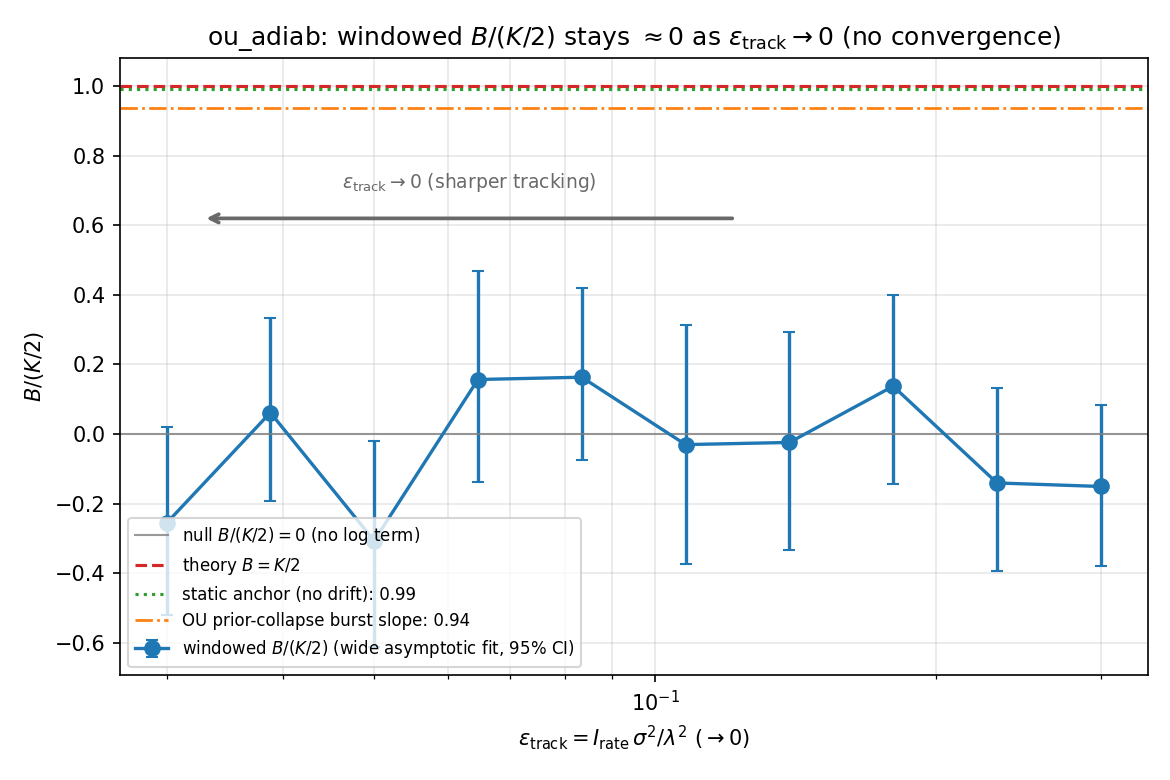
\includegraphics[width=0.82\linewidth]{figs/fig_ou_adiab_B_vs_eps.png}}

\caption{Structural unattainability of the \(K/2\) slope (C1, Proposition 1; series \protect\texttt{ou\_adiab}). The ratio \(B/(K/2)\), estimated in the wide asymptotic window, stays flat around zero as \(\epsilon_{\text{track}}\) is lowered by an order of magnitude --- rather than rising toward \(1\) --- whereas the static anchor (no drift) gives \(K/2\) (\(0.990\)), and the transient prior-collapse burst gives \(0.936\). The asymptotic fit window is \(\sigma\)-invariant (\(W \approx 156\)--\(166 \approx\) const across all 10 points, \(= c_0/(6\lambda r)\); the \(W\) values are given in § 6.1 and are not plotted), so the limit \(\epsilon_{\text{track}}\to0\) does not shift the fit from the plateau toward the transient logarithm. The grey line is the null hypothesis \(B/(K/2)=0\) (no log-term); all points sit on it.}

\end{figure}



\emph{2. \texttt{fou\_floor} --- the nostalgia floor and rate exponent for fractional OU (Theorem 2).} A real trajectory simulation on \textbf{exact stationary fOU} (not a recomputation of the closed-form formula): \(K = 56\) independent stationary fOU trajectories with \(H \in \{0.3,\ 0.5,\ 0.7,\ 0.9\}\) are generated by a \textbf{spectral-circulant method} from the density \(S(\omega) \propto |\omega|^{1-2H}/(\lambda^2+\omega^2)\); the Davies--Harte circulant eigenvalues are non-negative by construction (zero-clipping), the target autocovariance \(\gamma(k)\) being the inverse DFT of these eigenvalues. A \textbf{covariance control} confirms \(\hat\rho(s) \approx \gamma(s)\) (relative error \(<5\%\) up to lag \(\sim200\)--\(400\)). FIFO memory at \(\tau_E = 200\), \(c \approx 0.3\), \(|M| = 400\); a bit is predictive as long as \(\hat\rho^2(\text{age}) \ge \hat\rho^2(\tau_E)\).



\emph{Actual run result (seed 20260527, 40 realizations, path \(3.3\cdot10^4\), circulant \(M = 6.6\cdot10^4\)):} for all \(H\) --- the same floor \(\liminf\nu = 0.700 \approx 1-c\) (spread across \(H\) exactly \(0.000\); Fig. S2). An honest caveat about the \emph{status of the evidence}: this floor is set \emph{by construction} --- the deterministic threshold \(\hat\rho^2(\text{age}) \ge \hat\rho^2(\tau_E)\) pins the floor to \(1-c\) identically, so the zero spread is a consequence of the pinning, not an independent measurement (proof --- § S2). The independent content of \texttt{fou\_floor} is not the floor value but (i) the covariance control (genuine stationary fOU, not a surrogate) and (ii) confirmation of the \emph{exponent} \(4(1-H)\) in the far tail.



\textbf{The rate exponent \emph{agrees} with the analytical \(4(1-H)\)} (Fig. 2) --- on the correct process, in the far tail, from the exact covariance \(\gamma\) (the sample ACF on long memory is biased toward zero at large lags). In the far window (\(\Delta \gtrsim 8\tau_E\)) the local log-log slope of \(\rho^2\) matches \(4(1-H)\), and the two \(H\) play different evidential roles: \(H = 0.7\) (\(H < 3/4\), \(\int\beta_v\) finite) --- \emph{inside} the strict Theorem 2, the match \(1.237\) on \([8,40]\tau_E\) and \(1.201\) on \([20,80]\tau_E\) (analytic \(1.2\)) --- a \emph{within-theorem confirmation}; \(H = 0.9\) (\(H \ge 3/4\), \(\int\beta_v\) diverges) --- \emph{outside} the theorem, the match \(0.406\) and \(0.385\) (analytic \(0.4\)) --- only a \emph{numerically-supported conjecture}. In the near window \([\tau_E, 8\tau_E]\) the exponent is not isolated (\(1.62\) at \(H = 0.7\), \(0.46\) at \(H = 0.9\) from the exact covariance --- the OU ``knee''; \(2.44\) and \(1.40\) from the sample ACF --- estimator bias). \textbf{The exponent requires exact fOU generation:} the naive surrogate AR(1)\(\circ\)fGn would give \(2.23\) and \(1.26\), outside the CI of \(4(1-H)\) --- a surrogate artifact, not a property of the theory; on exact fOU both the depth \((1-c)\) and the exponent are reproduced. The qualitative dichotomy holds: at \(H = 0.5\) the tail is exponential (rate \(4.07\cdot10^{-3}\)/step), at \(H > 0.5\) it is power-law. \emph{Falsifier:} a far-tail exponent outside \(4(1-H)\) (not observed; a divergence of the floor \emph{depth} across \(H\) in \texttt{fou\_floor} is impossible by construction --- pinning by the threshold \(\hat\rho^2(\tau_E)\) --- so the independent falsification of the depth is carried by \texttt{psp\_floor}, § 6.3). The load-bearing C2 contribution --- the \emph{depth} \((1-c)\) --- is reproduced invariantly across \(H\); the exponent is secondary and asymptotic (§ 7 item vi).



\begin{figure}

\centering

\pandocbounded{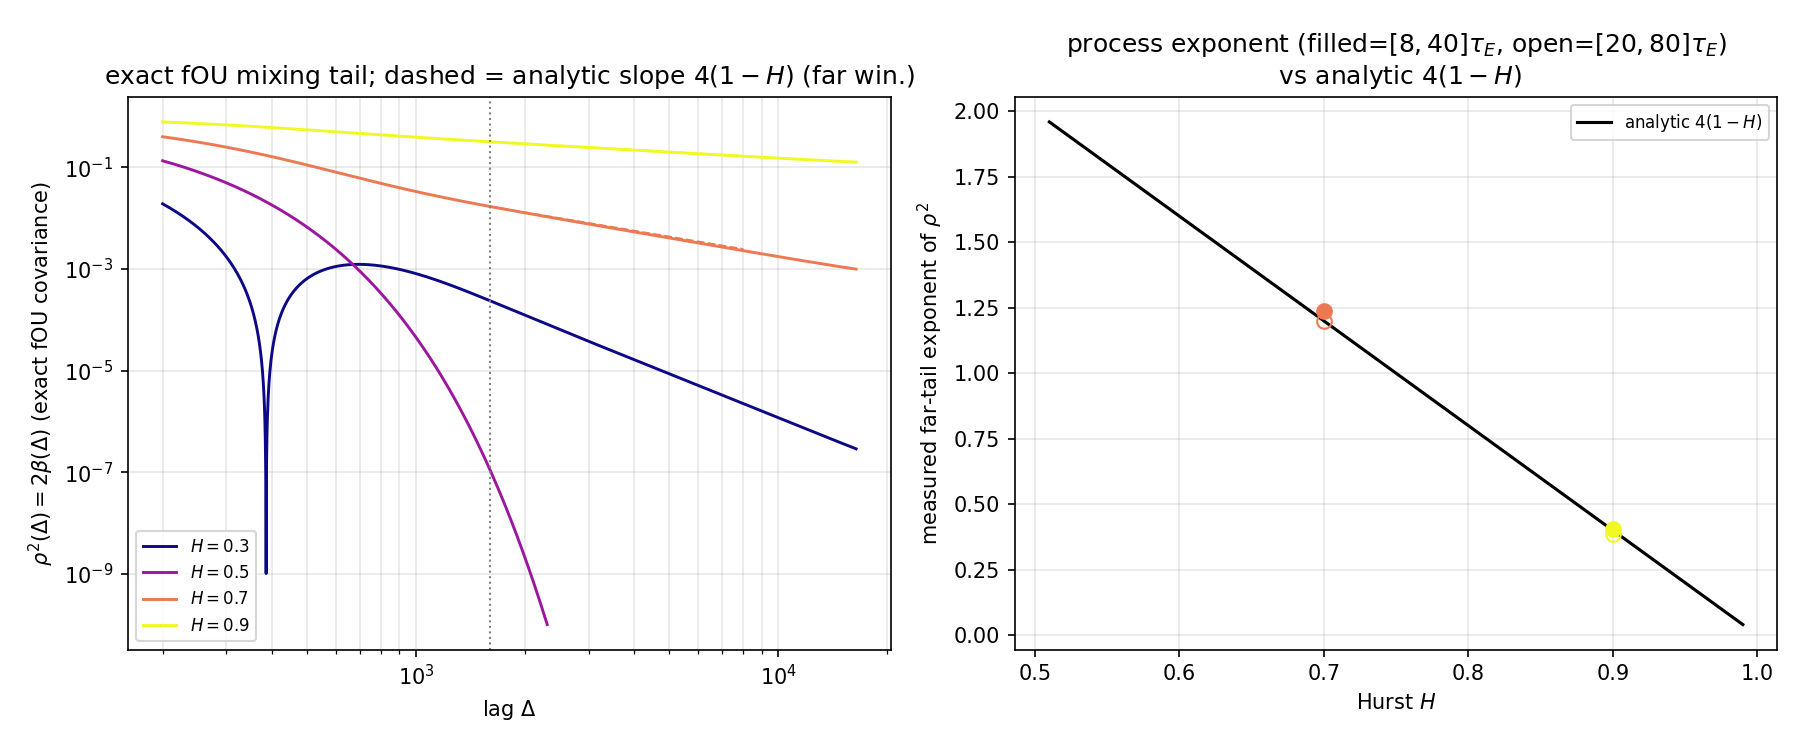
\includegraphics[width=0.82\linewidth]{figs/fig_fou_approach.png}}

\caption{Undertow rate exponent \(4(1-H)\) for fractional OU (C2, Theorem 2; series \protect\texttt{fou\_floor}). The tail \(\rho^2(\Delta) = 2\beta_v(\Delta)\) from the exact covariance for \(H \in \{0.3;0.5;0.7;0.9\}\); the far-tail log-log slope matches the analytical \(4(1-H)\) (within-theorem at \(H = 0.7\): \(1.24/1.20\); a numerically-supported conjecture at \(H = 0.9\): \(0.41/0.39\)). At \(H = 0.5\) the tail is exponential (OU control). The exponent is \emph{asymptotic far-tail}: beyond the OU ``knee'', not in the smallest window. The floor depth is invariant across \(H\) and is deferred to § S4.2 (Fig. S2).}

\end{figure}



\emph{3. \texttt{psp\_floor} --- the nostalgia floor for Poisson reset (Theorem 2).} A real trajectory simulation of the PSP surrogate of § 6.1 \cite{Andriishin2026b}: each coordinate carries a \emph{realized} Poisson stream of resets of intensity \(\mu = 1/\tau_E\); a retained bit is predictive until its coordinate has actually reset. The floor and the decorrelation rate are read from the realized process, not from the formula \(e^{-\mu\Delta}\). \emph{Actual run result (seed 20260528, 40 realizations, \(|M| = 400\), \(c \approx 0.3\), \(\mu \in \{10^{-3},\,3\cdot10^{-3},\,10^{-2}\}\)):} the settled empirical floor \(\hat\nu_{\text{floor}} = 0.709\text{–}0.713 \approx 1-c\) over a 10-fold range of \(\mu\) (spread \(0.004\); Fig. 3) --- invariance to the switching frequency is confirmed. Here the reset is a \emph{realized} stream, not a hard-wired threshold, so the floor \(0.709\text{–}0.713\) is \emph{independent} evidence (systematically slightly above the theoretical \(0.70\)). The decorrelation rate from the realized survival curve \(\hat S(\text{age})\) equals \(1.01\cdot10^{-3},\,3.01\cdot10^{-3},\,1.00\cdot10^{-2}\), each bootstrap CI covering the nominal \(\mu\) --- a genuine measurement of the scale \(1/\mu\). Together \texttt{psp\_floor} (exponential \emph{rate} \(\mu\)) and \texttt{fou\_floor} (power-law \emph{exponent} \(4(1-H)\)) exercise both ends of the mixing class. \emph{Falsifier:} dependence of the floor on \(\mu\) at fixed \(c\); a decorrelation rate outside the CI of \(\mu\) (not observed).



\begin{figure}

\centering

\pandocbounded{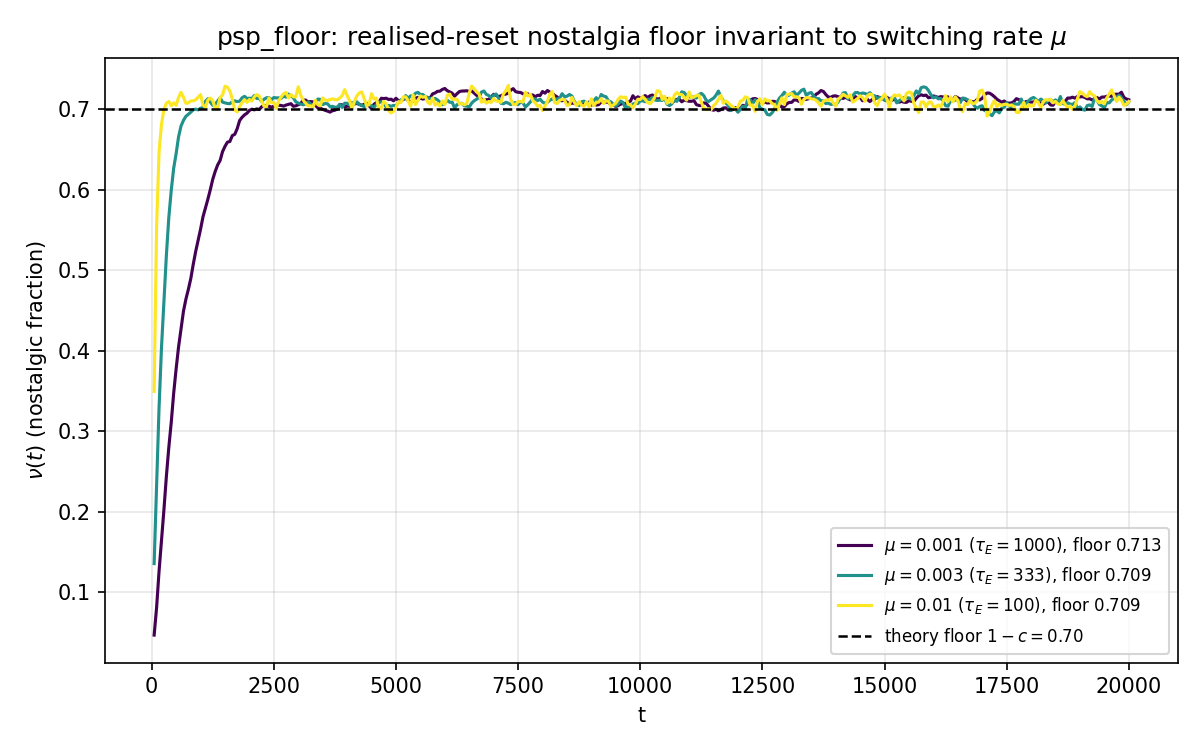
\includegraphics[width=0.82\linewidth]{figs/fig_psp_nu_vs_mu.png}}

\caption{Invariance of the nostalgia-floor depth across the refresh rate (C2, Theorem 2; series \protect\texttt{psp\_floor} --- \emph{independent} evidence). The settled floor \(\nu \approx 0.709\)--\(0.713 \approx 1-c\) is the same for Poisson-reset intensity \(\mu\) over a 10-fold range (\(\tau_E = 1/\mu \in \{1000,333,100\}\)), even though the \emph{approach dynamics} to the floor differ with \(\mu\) (three distinct curves are visible). Unlike the by-construction floor of \protect\texttt{fou\_floor} (Fig. S2), here the reset is a \emph{realized} Poisson stream, so the floor lies slightly above the theoretical \(0.70\) --- an independent measurement of the depth. The depth is set by the refresh rate \(c\), not by the drift frequency.}

\end{figure}



\emph{4. \texttt{superlinear\_memory} --- the phase boundary (Theorem 3).} Memory grows as \(|M_{\le t}| \propto t^\alpha\) for \(\alpha \in \{1,\ 1.5,\ 2,\ 3\}\) and separately exponentially \(e^{\kappa t}\); \(\nu(t)\) and the fresh fraction \(\phi(t)\) are measured. \emph{Actual run result (seed 20260529, \(\tau_E = 200\)):} for all polynomial \(\alpha\) the fresh fraction \(\phi(t) \sim t^{-\gamma}\) with \(\gamma \in \{1.000;\,0.991;\,0.982;\,0.964\}\) on the baseline window, and the prefactor \(\phi\cdot t \to \alpha\tau_E\) (\(200,\,298,\,394,\,581\) versus \(200,\,300,\,400,\,600\)): the fresh fraction vanishes for any finite \(\alpha\), whence structurally \(\eta_v \to 0\) (inflation of \(I_{\text{mem}}\)) --- there is no polynomial \(\alpha_c\) (Fig. 4). \emph{Caveat about circularity (important).} The \(\nu(t) \to 1\) shown in this series is an \textbf{artifact of the threshold model} ``a bit is useful \(\Leftrightarrow\) age \(< \tau_E\)'' (§ S4.4): the threshold hard-wires per-bit uniformity and \emph{forbids} a joint estimate of \(\theta_v(t)\) from fresh snapshots, so its \(\nu \to 1\) does \emph{not} test the claim about \(\nu^{\text{theor}}\) (which by § S1.6 / § S3.2 gives \(\nu^{\text{theor}} \to \nu_{C1} < 1\), not \(1\)). The series illustrates precisely the mechanism \(\eta_v \to 0\) / inflation of \(I_{\text{mem}}\); testing the \(\nu^{\text{theor}}\) plateau at the \(\nu_{C1}\) level requires a real joint Kalman estimate over the fresh FIFO subset --- this is done by the separate series \texttt{superlinear\_noncirc} (item 4a; § S4.4a). The leading exponent is identically \(\gamma = 1\); the downward drift of \(\gamma\) with growing \(\alpha\) is finite-window subleading curvature \(\phi = 1-((t-\tau_E)/t)^\alpha\), removed by widening the window: \(\times10\) gives \(\gamma \to \{1.000;\,0.999;\,0.998;\,0.996\}\), \(\times1000\) --- all \(1.000\) (diagnostic \texttt{gamma\_window\_convergence}, § S4.4). For exponential growth (\(\kappa\tau_E \in \{0.1;\,0.5;\,1\}\)) --- \(\phi_\infty = 1-e^{-\kappa\tau_E} \in \{0.095;\,0.394;\,0.632\} > 0\) (nostalgia below \(1\)), but the capacity \(|M_{\le t}| \propto e^{\kappa t}\) diverges (the ratio \(|M_{\le T}|/|M_{\le 0}|\) up to \(9.8\cdot10^{42}\)), without raising the horizon-bounded \(I_{\text{pred}} \le H_\tau\) (5.3), so that \(\eta_v(t) = I_{\text{pred}}/I_{\text{mem}} \to 0\) structurally (a bounded numerator over a growing denominator) --- \emph{for an informational, not an energy-budget, reason}: the run records a \emph{capacity-estimate} \(\eta_v(T)/\eta_v(0) \in \{5\cdot10^{-5};\,3\cdot10^{-22};\,10^{-43}\}\) for \(\kappa\tau_E \in \{0.1;\,0.5;\,1\}\) --- this is the inverse capacity ratio \(|M_{\le 0}|/|M_{\le T}|\) (in the run \(I_{\text{mem}}\) was taken \(\propto |M_{\le t}|\), \(I_{\text{pred}} = H_\tau\)), i.e., a \emph{conservative upper estimate} of the decay of \(\eta_v\). The true \(I_{\text{mem}} \le H(X_E^{\le t})\) grows only \(\sim\)linearly (§ S3.4), so the actual decay of \(\eta_v\) is slower than the capacity one (of order \(1/t\)) --- but the limit \(\eta_v \to 0\) is the same, there is no escape (an illustration, not a measured MI). \emph{Falsifier:} a \(\nu^{\text{theor}}(t)\) reaching a floor \emph{below \(1\)} at some finite polynomial \(\alpha\) (under satisfied mixing and per-bit uniformity) would refute the absence of \(\alpha_c\). The testable content is in the DPI-transfer S2.0 (\(\phi(t)\to0 \Rightarrow \nu^{\text{theor}}\to1\)), not in \(\phi\sim\alpha\tau_E/t\) itself, which is an identity of the expansion (§ 5 item 5a); the observed downward drift of \(\gamma\) is a finite-window artifact of this identity, not a test of the theorem.



\begin{figure}

\centering

\pandocbounded{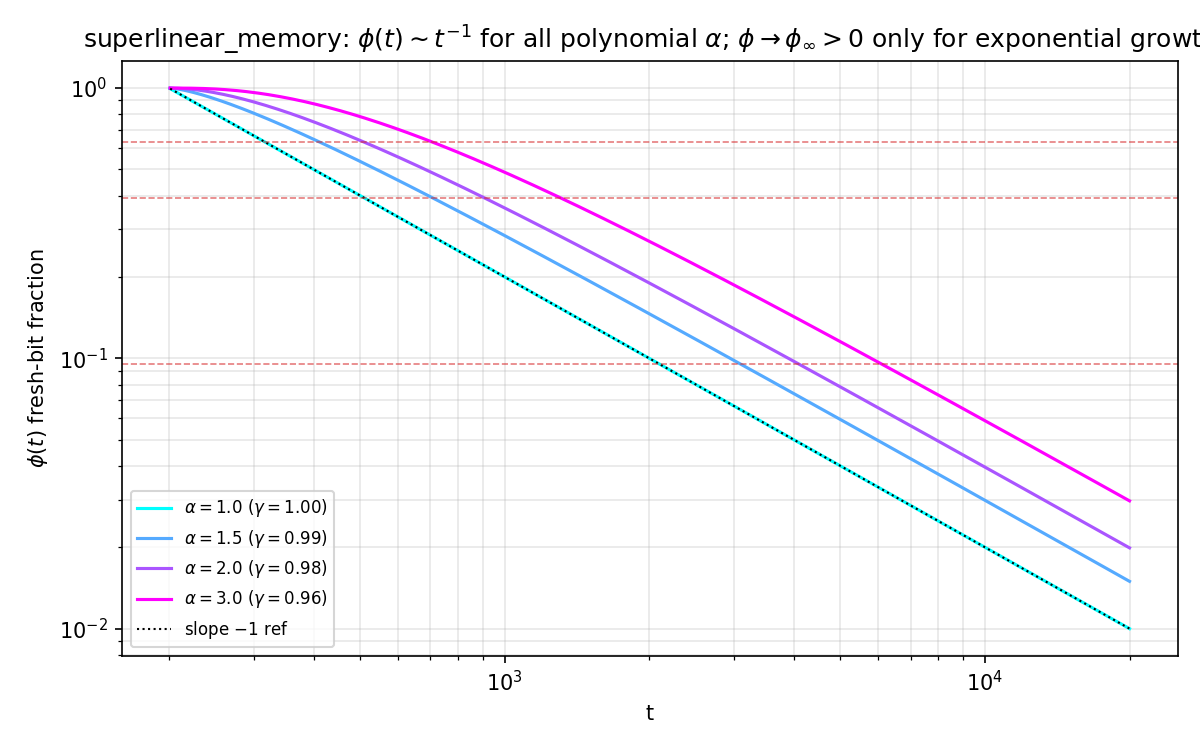
\includegraphics[width=0.82\linewidth]{figs/fig_superlinear_phi.png}}

\caption{Absence of a finite polynomial threshold \(\alpha_c\) (C3, Theorem 3; series \protect\texttt{superlinear\_memory}). The fresh-bit fraction \(\phi(t) \sim t^{-\gamma}\) has leading exponent \(\gamma \equiv 1\) for all polynomial \(\alpha \in \{1;1.5;2;3\}\) (prefactor \(\phi\cdot t \to \alpha\tau_E\)), whence structurally \(\eta_v \to 0\) (inflation of \(I_{\text{mem}}\)) --- the route is closed for any finite \(\alpha\). The shown \(\nu \to 1\) is an artifact of the threshold model (§ S4.4); the true \(\nu^{\text{theor}} \to \nu_{C1} < 1\) (§ S1.6). The visible downward drift of \(\gamma\) with growing \(\alpha\) on the original window is a finite-window subleading artifact of the exact \(\phi = 1-((t-\tau_E)/t)^\alpha\), removed by widening the fit window (convergence diagnostic, § S4.4). Escape is possible only through exponential capacity growth --- Fig. S5.}

\end{figure}



\emph{4a. \texttt{superlinear\_noncirc} --- non-circular confirmation of the \(\nu^{\text{theor}}\) plateau at the C1 floor (Theorem 3).} This series fixes the circularity of the threshold model of \texttt{superlinear\_memory}: the learner builds a \emph{real joint Kalman posterior} over the current \(\theta_t\) from a growing fresh FIFO subset (with no age gate), so that the fresh snapshots of one coordinate \emph{jointly} estimate \(\theta_v(t)\) down to the tracking floor \(\Sigma_\infty\). The model is an A1 linear-Gaussian representative of the softmax chain (§ S3.2): \(X_{t+1} = \theta_t X_t + w\) with the \(\theta_t\) coupling by OU, observed only multiplicatively (\(K = 56\), \(\lambda = 0.1\), \(\sigma^2 = 2\cdot10^{-3}\), seed \(20260527\)). \emph{Actual run result:} at \(\epsilon_{\text{track}} = 0.204\) the theoretical nostalgia reaches a \textbf{plateau \(\nu^{\text{theor}} = 0.96\)} (Fig. 5), coinciding with the analytical C1 floor \(\nu_{C1} = \Sigma_\infty/\sigma_0^2 = 0.95\) (§ 5 item 2, § S3.2), and \textbf{\(\alpha\)-independent} (for \(\alpha \ge 1\) FIFO retains the whole history, the floor \(\Sigma_\infty\) is unbeatable --- no polynomial \(\alpha\) shifts the plateau); the estimate \(\hat\Sigma \to \Sigma_\infty = 0.0101\) reaches \emph{the floor}, not zero. The sanity controls are exact (no memory \(\nu = 1.000\), oracle \(\nu = 0.000\)). The load-bearing evidence is the \emph{divergence}: the naive per-bit majorant \(\nu_{\text{naive}} = 1-\phi \to 1\) (the old circular \texttt{superlinear\_memory} result) diverges from the real plateau \(\nu^{\text{theor}} \to \nu_{C1} < 1\), whereas \(\eta_v \to 0\) (the decoupling of \(\nu^{\text{theor}}\) and \(\eta_v\), § 5 item 4). Thereby the \(\nu \to 1\) of the threshold model (Fig. 4) is directly exhibited as an artifact of circularity. \emph{Falsifier:} a \(\nu^{\text{theor}}\) plateau at the level of \(1\) (rather than \(\nu_{C1}\)) under a saturated fresh influx would refute the C1 floor --- not observed (plateau \(0.96 \approx \Sigma_\infty/\sigma_0^2\)).



\begin{figure}

\centering

\pandocbounded{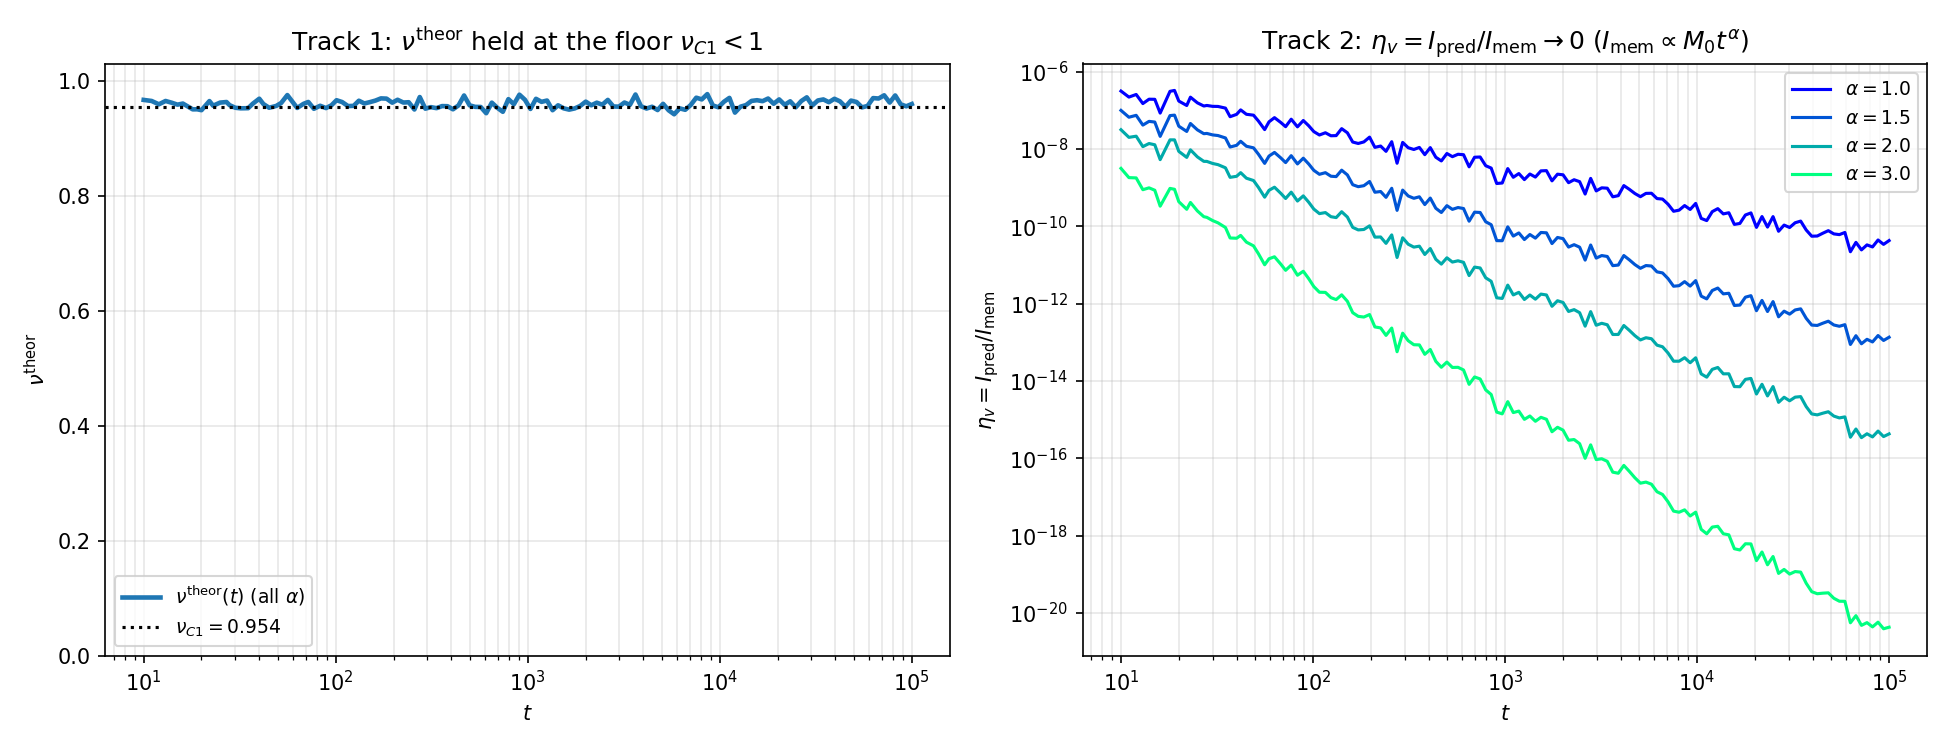
\includegraphics[width=0.82\linewidth]{figs/fig_noncirc_two_track.png}}

\caption{The non-circular \protect\texttt{superlinear\_noncirc} series (a real joint Kalman posterior over the fresh FIFO, with no age gate). \emph{Left:} the theoretical nostalgia \(\nu^{\text{theor}}\) is held at a plateau at the C1 tracking floor \(\nu_{C1} = 0.954 < 1\) --- flat and \(\alpha\)-independent (the curves for \(\alpha \in \{1;\,1.5;\,2;\,3\}\) coincide: the FIFO retains the entire history). \emph{Right:} the efficiency \(\eta_v = I_{\text{pred}}/I_{\text{mem}} \to 0\) (with \(I_{\text{mem}} \propto M_0 t^\alpha\)), the faster the larger \(\alpha\). It is this separation that closes the capacity-growth route: nostalgia stays below \(1\) while \(\eta_v\), not \(\nu^{\text{theor}}\), goes to zero (§ 5 item 4).}

\end{figure}



\emph{5. What the simulations do not do.} (i) They do \emph{not} prove the theorems --- these are illustrations; the rigorous statements are carried by § S1--S3. (ii) They work only with a known true \(\theta_v(t)\), hence \(\nu^{\text{theor}} = \nu^{\text{op}}\) by construction \cite{Andriishin2026b} § 6; the operational indistinguishability of the two normalizations is not tested. (iii) They do not go beyond abstract Markov chains with logit drift. (iv) Convergence \(B \to K/2\) is checked on a finite scan --- support, not proof. (v) The class of non-mixing (heavy-tailed) environments is not simulated --- outside the domain of Theorem 2.



\section{Discussion}\label{discussion}



\emph{1. Connection to non-stationary online learning.} The cumulative excess loss \(L_{\text{excess}}(t)\) is the dynamic regret relative to an oracle tracking the drifting optimum. Two budgets of change: (i) the \emph{path length} \(P_T = \sum_t \|\theta_v(t)-\theta_v(t-1)\|\) \cite{Zinkevich2003} with the bound \(O(\sqrt{T}(1+P_T))\) against a drifting comparator (Hall--Willett \cite{HallWillett2015} --- dynamic mirror descent; the tight \(O(\sqrt{T(1+P_T)})\) with a matching lower bound --- Zhang--Lu--Zhou \cite{ZhangLuZhou2018}); (ii) the \emph{variation budget} \(V_T\) in the minimax theory of Besbes--Gur--Zeevi \cite{BesbesGurZeevi2015}, \(\Theta(T^{2/3}V_T^{1/3})\). For smooth OU drift both budgets grow linearly (\(P_T, V_T \propto T\)): BGZ gives a linear \(\Theta(T)\), Hall--Willett a dominating \(O(T^{3/2})\); for \emph{strongly-convex} losses the tight bound \(O(P_T)\) \cite{Mokhtari2016} gives exactly \(\Theta(T)\). All this is compatible with the linear term \(A\cdot t\) (3.1) (certified by the stationary Riccati \(\Sigma_\infty > 0\), § S1.2); our model is quadratic (§ S1.3), so the strongly-convex line is the relevant one. The refinement of Theorem 1 concerns not the leading \(\Theta(T)\) but the \emph{sub-linear} logarithmic correction \((K/2)\ln(\lambda t)\) --- which saturates into a plateau (Proposition 1); \emph{logarithmic} regret is attained for strongly-convex losses \cite{Hazan2007,HazanSeshadhri2009}, which our \((K/2)\ln\)-asymptotics is closer to. The difference of forms (power-law BGZ versus logarithmic) reflects the difference of settings: BGZ bound the \emph{total} variation, we bound the \emph{spectral} structure of the drift (the role of mixing, the scale \(\tau_f^{\text{forget}}\) below \(\tau_E\); monotonicity in \(\tau_E\) \cite{Andriishin2026b} § S5.4). The connection with \(\eta_v = I_{\text{pred}}/I_{\text{mem}}\) and \(\nu\) through the identity ``regret = excess-loss = unpaid predictive value'' \cite{CesaBianchiLugosi2006,Hazan2007} deserves a separate study.



\emph{1a. The necessity of restricting the class.} Theorem 2 extends the domain of the floor but does not cancel the fundamental limitation: without a prior restriction of the drift class, sub-linear dynamic regret is unattainable --- under an unbounded variation budget every learner incurs regret no slower than linear \cite{BesbesGurZeevi2015,Zinkevich2003}. The mixing condition (4.1) is a necessary restriction: it selects environments that forget their past; outside it (heavy-tailed, non-recurrent drift) neither the floor \(1-c\) nor the adiabatic asymptotics are guaranteed. The boundary of the admissible class of § 4 is not a defect but a reflection of this impossibility: the undertow is inevitable for mixing environments --- the natural class of environments that forget their past --- where mixing is a \emph{sufficient} condition, not a provably-maximal class (broader sufficient conditions remain open). In the philosophical background this is in the spirit of no-free-lunch \cite{Wolpert1996}, but formally we do not rely on NFL (the load-bearing argument is the impossibility of sublinear dynamic regret); moreover, \cite{Wolpert1996} is NFL of \emph{supervised} learning, averaging over classes of target functions, not over \emph{environments} with a fixed spectral structure, so it is applicable only as an analogy.



\emph{1b. Delineation from related notions.} To avoid rebranding, we distinguish three notions. \emph{Nostalgia} is the retention of an obsolete memory layer that no longer predicts anything but \emph{continues to be paid for} thermodynamically. \emph{Catastrophic forgetting} \cite{McCloskeyCohen1989,Kirkpatrick2017} is the opposite pathology: the \emph{loss} of still-useful memory during continued training. \emph{Concept drift} \cite{Gama2014} is a property of the \emph{environment} itself (a shift of the distribution), a cause, not a consequence. Nostalgia does not reduce to them: it is the thermodynamic cost of \emph{successful} retention (unlike forgetting) under drift (concept drift as an external cause), and its subject is that retention fails to pay for itself, not the preservation or loss of information.



\emph{2. Kalman tracking.} The EWMA filter of Theorem 1 is a special case of the stationary Kalman--Bucy filter for a linear-Gaussian system with a hidden OU state \cite{KalmanBucy1961,AndersonMoore1979}; the stationary error \(\Sigma_\infty \propto \sigma^2/\lambda\) (the root of the algebraic Riccati equation) is transferred into the thermodynamic context as the linear coefficient \(A\). The nonzero \emph{steady-state tracking floor} itself is the classical \emph{lag misadjustment} of adaptive filtering \cite{Widrow1976,Haykin2014}. Our contribution is not the existence of the floor but its thermodynamic reading (the floor \(\Leftrightarrow\) the linear term \(A\) and the plateau of the logarithm) and its role as an informational lower bound on \(n_{\text{eff}}\) (§ S1.6). Generalization to the nonlinear softmax model (extended/unscented Kalman) is a technical extension, parallel to Remark 6 \cite{Andriishin2026b}.



\emph{3. Renewal theory.} The PSP class of Theorem 2 is a renewal process: the reset points form a Poisson stream, the ages of the bits are residual lifetimes. The uniformity of the age distribution under FIFO (§ 4.2, § S2.0) is a consequence of the \emph{stationary age distribution} of a fixed-size buffer (inspection paradox / backward recurrence time, \cite{Cox1962} ch.~5), and \emph{not} of the elementary renewal theorem. The power-law mixing of fOU at \(H > 1/2\) corresponds to heavy-tailed renewal --- a natural continuation.



\emph{4. What remains open.} (i) \emph{Heavy-tailed and non-Markovian drift without mixing}: Theorem 2 requires \(\beta_v(s) \to 0\); environments with a divergent autocorrelation fall out of the class, and the floor \(1-c\) is not guaranteed for them. (ii) \emph{A bridge to fluctuation theorems}: the cumulative Still bond (§ 2.1) can be refined by the Jarzynski theorem with feedback \cite{SagawaUeda2010}, by inequalities for bipartite systems and transfer entropy \cite{HartichBaratoSeifert2014}, by the stochastic thermodynamics of computation \cite{Wolpert2019} (review --- \cite{Parrondo2015}). It is essential that the C2 floor does \emph{not} transfer into a drift-dependent lower estimate of the dissipation \emph{rate} by direct substitution into the step-wise bond: the Still bond carries the instantaneous non-predictive information about the \emph{present} signal, from which the obsolete layer (the carrier of the trajectory-level \(\nu^{\text{theor}}\to1\)) is decorrelated by mixing (4.1) and hence thermodynamically \emph{mute}; the honest form without a drift-dependent \((1-c)\) is the stationary limit \(t^{-1}\langle W_{\text{diss}}^{[0,t]}\rangle \ge k_B T\,\overline{I_{\text{nonpred}}^{\text{inst}}} > 0\) \cite{Andriishin2026b} § S9.4, while a drift-\emph{dependent} estimate requires a separate argument (a feedback fluctuation theorem) and remains open. (iii) \emph{Operational versus theoretical nostalgia}: Theorem 1 gives asymptotics for the counterfactual \(L_{\text{excess}}\); the transfer to the measurable operational nostalgia \(\nu^{\text{op}}(t)\) remains structural (the DPI direction is reversed, § 2.2). (iv) \emph{A rigorous transient filter}: the derivation of \(K/2\) relies on the stationary Riccati and the heuristic \(n_{\text{eff}} \asymp \lambda t\) (A3); the rigorous non-stationary Riccati and control of the softmax-linearization remainder (A1) beyond the adiabatic window are open. (v) \emph{Numerical asymptotic realizability of \(B \to K/2\) (established as unattainable)}: the extended check with an \emph{optimal} Kalman learner (§ 6.1, § S4.1) refutes the working hypothesis --- the attempt to push \(\epsilon_{\text{track}} \to 0\) in order to recover \(\hat B \to K/2\) as a slope (it is precisely the attempt that is refuted, \emph{not} the hypothesis of § S8.1 \#2 \cite{Andriishin2026b}, which Theorem 1 analytically confirms). Under genuine OU drift \(n_{\text{eff}}\) is bounded by the floor \(1/g^\star\), \(L_{\text{excess}}\) reaches a plateau, and \(B/(K/2) \to 0\) in any wide window at any \(\sigma\); the obstruction is structural (the \(\sigma\)-invariance of the fit window, Proposition 1, § 6.1). Growing memory does not help --- the floor is the MMSE lower bound on \(n_{\text{eff}}\) across all architectures (§ S1.6, § 3). Therefore the question of growing memory is neither ``open'' nor ``closed onto C3'', but \emph{removed} by the optimality of the floor in the A1 window (the non-Gaussian model is open, item iv). (vi) \emph{Empirical rate exponent of the fOU undertow}: the load-bearing C2 contribution --- the \emph{depth} of the floor \((1-c)\) --- is proved and does not depend on the rate exponent; the \emph{exponent} \(4(1-H)\) is secondary and \emph{asymptotic} --- on exact stationary fOU it is confirmed in the far tail (\(\Delta \gtrsim 8\tau_E\): \(1.20\) at \(H = 0.7\) versus the analytic \(1.2\); \(0.39\)--\(0.41\) at \(H = 0.9\) versus \(0.4\)), but in the near window it is not isolated (the OU ``knee'', the biased sample ACF), and is read off the exact covariance (§ 6.2, § S4.2). Structurally this is the \emph{same situation as the transience in C1}; on correct fOU (not the AR(1)\(\circ\)fGn surrogate) both the depth \((1-c)\) and the exponent are reproduced, which \textbf{strengthens} C2. Only a rigorous control of the convergence rate at \(H \ge 3/4\) remains open --- this does not undermine the floor.



\section{Relation to prior work}\label{relation-to-prior-work}



The present work is the third step of the program on the informational efficiency of self-modeling \(\eta_v = I_{\text{pred}}/I_{\text{mem}}\) (the Landauer motif, the thermodynamic Still anchor) and extends, rather than revises, both predecessors.



\emph{Formula-free summary.} The undertow is inevitable for one simple reason: all three ways of escaping it run up against the same thing. Old knowledge inevitably ceases to correlate with the present --- the environment forgets its past, and with it the memory recorded about that past is devalued. Therefore neither more precise tracking, nor faster refresh, nor capacity growth save the situation: behind the three closed routes stands one mechanism --- the \emph{decorrelation of old memory}. One has to pay more and more for storing devalued memory, but this growing cost is already a \emph{consequence} (the structural smallness of efficiency), not a second independent mechanism.



\emph{Closure of the three routes.} The three theorems close three escape routes, all three dead ends (precise tracking --- the no-go of realizability of Proposition 1; memory refresh --- the universal floor \(1-c\) of Theorem 2; capacity growth --- the absence of a polynomial threshold of Theorem 3), and jointly obsolescence is ineliminable: nostalgia \(\nu^{\text{theor}}\) is held at a nonzero floor (C2 \(1-c\) for fixed memory; C1 \(\nu_{C1} < 1\), to which it converges as the fresh budget of growing memory saturates), while efficiency \(\eta_v = I_{\text{pred}}/I_{\text{mem}} \to 0\) for any growing memory. Nostalgia need not reach \(1\) here: the load-bearing inevitability of the capacity-growth route is the vanishing of \(\eta_v\), not \(\nu^{\text{theor}} \to 1\) (§ 5 item 4).



The routes are closed not \emph{independently} but \emph{interlockingly}, which removes the objection that the inevitability is conditional --- ``only for saturating memory'', whereas a learner with \emph{growing} memory would raise \(n_{\text{eff}}\) above the floor \((1-g^\star)/g^\star\). The floor is the \emph{tracking optimum} --- a lower bound on \(n_{\text{eff}}\) across all memory architectures in the linear-Gaussian A1 window (§ 7 item iv, item v; § S1.6; the non-Gaussian case is open), so an attempt to raise \(n_{\text{eff}}\) is either informationally futile (the optimal filter is already at the floor --- C1, the same decorrelation mechanism \(\beta_v(\Delta t)\to0\) that carries the C2 floor)\footnote{The floor concerns decorrelation from the \emph{current} \(\theta_v(t)\), whereas the mechanism of Theorem 2 (4.1) concerns decorrelation from the \emph{future trajectory} \(\theta_{[t,t+\tau]}\); for a horizon \(\tau = O(1)\) both have the same decay exponent (for fOU the trajectory supremum is attained at the near end, preserving the leading \(4(1-H)\)). The full argument --- § S2.0, the Remark ``trajectory versus pair''.}, or suboptimal by piling up raw material (the regime of Theorem 3: growth of \(|M_{\le t}|\) does not raise the horizon-bounded \(I_{\text{pred}}\), while a growing \(I_{\text{mem}}\) drives \(\eta_v \to 0\)). Growing memory \emph{does not open} a fourth route.



The independent contribution of the work is not in a separate result (each brick is attributed: § 3 item 6, § 4 item 3, § 5 item 5a), but in \emph{closing the loop}: the floor of \emph{nostalgia} along all three routes is set by \emph{decorrelation} (mixing) --- it carries both the C2 floor (\(1-c\)) and the C1 floor (\(\nu_{C1}\)), to which \(\nu^{\text{theor}}\) converges even with growing memory; the closing of precisely the \emph{capacity-growth} route is carried by the structural smallness of \(\eta_v\) (§ 5 item 4), which does not itself give a quantitative floor on nostalgia. The closure itself is a testable prediction --- the vanishing \(\hat B \to 0\) in a wide window (§ 6), which is confirmed. Beyond paper \#2 three things are strictly new: (i) the DPI-generalization of the floor from the OU spectral gap to general mixing (capturing non-Markovian fOU through multiple, not pairwise, correlation --- § 4); (ii) the polynomial/exponential phase boundary and the structural smallness of \(\eta_v\) in the exponential limit as an answer to § 8.5 \#2 \cite{Andriishin2026b} (§ 5 item 4); (iii) the demonstration that the three routes are \emph{not} independent --- they reduce to one mechanism.



Level qualifier: the no-go is conditional on assumptions (A1)--(A3) of Theorem 1 (softmax regularity \cite{Andriishin2026b} Remark 6; Bayesian class-II concentration \cite{BialekNemenmanTishby2001}) and on the linear-Gaussian adiabatic approximation; ``inevitability'' is proved \emph{in the adiabatic window} / \emph{for mixing environments} (\(\beta_v(\Delta t)\to0\), § 2.6, § 4) --- a rigorous version beyond the class (non-adiabaticity, heavy-tailed drift) is open (§ 4.6, § 7 items i, iv), while the full transfer to \emph{operational} \(\nu^{\text{op}}\) remains structural (the DPI direction is reversed, § 2.2, § 7 item iii). Within these bounds obsolescence is a structural property, not an artifact: the rational response is not to build up precision or capacity, but to periodically \emph{reset} the obsolete layer (the optimal \(\tau_{\text{reset}}^*\) \cite{Andriishin2026b} (12), § 5 item 6).



Nor does the quasi-stationary limit \(\lambda \to 0\), in which \(n_{\text{eff}} \sim t\) could grow (\(\tau_E \to \infty\)), form a fourth route: while adiabaticity is preserved it \emph{continuously degenerates into the stationary regime}, where there is no undertow \emph{by definition}, rather than the undertow being overcome (the growth \(n_{\text{eff}} \sim t\) is the vanishing of drift, and the floor \(1/g^\star \to \infty\) together with \(g^\star \propto \sigma^2 \to 0\)). Neither finite \(\lambda\) (the floor is active) nor \(\lambda \to 0\) (the drift vanishes) opens an escape.



\emph{Relation to paper \#2 \cite{Andriishin2026b}.} All three theorems advance the open questions of § 8.5 without coming into contradiction. Theorem 1 \emph{resolves} aspect (i) of the § S8.1 hypothesis \emph{negatively}: \(B = K/2\) is confirmed in the limit \(\epsilon_{\text{track}}\to 0\) \emph{as transient}, but there is no attainable asymptotic realization of the slope under drift (no-go, Proposition 1); the transfer to \(\nu^{\text{op}}\) is open (§ 7). Theorem 2 \emph{embeds} Lemma 2 as the special case \(H = 1/2\) (the OU spectral gap is a sufficient, not a necessary, condition; the necessary one is mixing (4.1)). Theorem 3 closes the question of superlinear memory: escape is impossible either polynomially or exponentially --- \(\eta_v\) is structurally negligible, while \(\nu^{\text{theor}}\) is held at the C1 floor (\(\nu_{C1} < 1\)). The apparatus of \cite{Andriishin2026b} is used without redefinition.



\emph{Relation to paper \#1 \cite{Andriishin2026a}.} The stationary result \cite{Andriishin2026a} § 2.1 is a special case of the non-stationary efficiency \(\eta_v = I_{\text{pred}}/I_{\text{mem}}\) in the zero-drift limit \cite{Andriishin2026b} § 2.1: there the \emph{drift-induced} nostalgia \(\nu \to 0\) and \(L_{\text{excess}}\) does not grow logarithmically, both theorems degenerating into the stationary picture. This \(\nu \to 0\) does \emph{not} cancel the ``nostalgia bits'' of result \#1 --- they are from a different mechanism (the finite-memory sink: retention beyond the correlation scale even without drift), which is nonzero also in the stationary limit. The mechanisms are orthogonal: the drift-induced undertow vanishes at zero drift, the finite-memory sink does not.



\emph{Progressiveness of the extension.} The program satisfies the Lakatosian criterion: each work adds excess, independently testable content (paper \#1 --- the stationary scale; \#2 --- the non-stationary extension; the present one --- three theorems that reduce three routes to a single thesis). The negative result (Proposition 1) is a \emph{progressive}, not a degenerative, shift: it does not save the § S8.1 hypothesis by an auxiliary patch but makes a confirmable prediction (\(\hat B \to 0\) in a wide window, § 6). New open problems (the convergence rate at \(H \ge 3/4\); heavy-tailed drift; a bridge to fluctuation theorems) remain for future works; the operationalization with \emph{growing} memory does not remain open --- it is closed by the optimality of the floor (§ 7 item v).



\emph{Substrate-independence.} The undertow is a property of the information thermodynamics of non-stationary memory, not of the substrate: neither the ceiling of the numerator (\(I_{\text{pred}} \le \ln k\)) nor the growth of the denominator \(I_{\text{mem}}\) (\(\le H(X_E^{\le t})\)) depends on whether the memory is stored in synapses, network weights, or an epigenetic mark. Hence a unified reading of why adaptive systems on different substrates converge to one strategy --- to periodically \emph{reset} the obsolete layer (continual learning with a \emph{finite} replay buffer, synaptic turnover, epigenetic reprogramming --- § 5 item 6, § 7 item 1b): candidates for the manifestation of a single no-go. This is a parallel, not a derivation --- the theorems are proved only in the model class (mixing slow drift, the A1 window), and verification on concrete systems remains a separate task.



\section*{Declarations}
\textbf{Funding.} No external funding was received for this research.



\textbf{Competing interests.} The author declares no competing interests.



\textbf{Author Contributions.} Sole author (A.A.): conceptualization, proofs, numerical design, and writing.



\textbf{Data Availability.} The numerical-simulation code (§ 6) and the source files of the work are openly available in the public mirror repository \texttt{andriishin/landauer-undertow-oa} (GitHub) and archived on Zenodo (DOI 10.5281/zenodo.21039220). The work uses no external empirical data (a theoretical work with numerical illustrations on abstract models).



\textbf{AI disclosure.} The author used an AI assistant (large language model) as a tool for drafting, literature cross-referencing, and editing under the author's direct supervision. All mathematical results, proofs, and scientific claims were conceived, verified, and approved by the author, who takes full responsibility for the content.




\section*{References}
\bibliographystyle{iopart-num}
\bibliography{refs}

\end{document}
